\documentclass[ms,english]{stthesis}

% --- Load packages START
\usepackage[T1]{fontenc}
\usepackage{libertinus}

\usepackage[utf8]{inputenc}
\usepackage[english]{babel}
\usepackage{isodate}

% Bibliography
\usepackage[
    style=numeric-comp,
    backend=biber,
    url=false,
    doi=false,
    isbn=false,
    hyperref,
]{biblatex}

\addbibresource{content/bibliography.bib}

\usepackage{hyperref} % makes all links clickable but hides ugly boxes
\usepackage[capitalise,nameinlink,noabbrev]{cleveref} % automatically inserts Fig. X in the text with \cref{..}
\usepackage{todonotes}
\usepackage{pdfpages} % to insert pdf pages
\usepackage{xcolor}
\usepackage{csquotes}

% insert python code snipets
\usepackage{listings}
\definecolor{codegreen}{rgb}{0,0.6,0}
\definecolor{codegray}{rgb}{0.5,0.5,0.5}
\definecolor{codepurple}{rgb}{0.58,0,0.82}
\definecolor{backcolour}{rgb}{0.95,0.95,0.92}

\lstdefinestyle{mystyle}{
	backgroundcolor=\color{backcolour},   
	commentstyle=\color{codegreen},
	keywordstyle=\color{magenta},
	numberstyle=\tiny\color{codegray},
	stringstyle=\color{codepurple},
	basicstyle=\ttfamily\footnotesize,
	breakatwhitespace=false,         
	breaklines=true,                 
	captionpos=b,                    
	keepspaces=true,                 
	numbers=left,                    
	numbersep=5pt,                  
	showspaces=false,                
	showstringspaces=false,
	showtabs=false,                  
	tabsize=2
}

\lstset{style=mystyle} % enable cref for listing
\crefname{lstlisting}{Listing}{listings}
\Crefname{lstlisting}{Listing}{Listings}

\lstnewenvironment{code}[1][]% use 'code' instead of 'lstlisting' to prevent splitting between pages
{
	\noindent
	\minipage{\linewidth} 
	\vspace{0.5\baselineskip}
	\lstset{basicstyle=\ttfamily\footnotesize,#1}}
{\endminipage}


\usepackage{caption}
\usepackage{subcaption}
\captionsetup{font=sf,labelfont=bf,labelsep=space}
\usepackage{floatrow}
\floatsetup{font=sf}
\floatsetup[table]{style=plaintop}
\captionsetup{singlelinecheck=off,format=hang,justification=centering}
\DeclareCaptionSubType[alph]{figure}
\DeclareCaptionSubType[alph]{table}
\captionsetup[subfloat]{labelformat=brace,list=off}

\usepackage{booktabs} % fancy tables. need to analyse.
\usepackage{array}
\usepackage{tabularx}
\usepackage{tabulary}
\usepackage{tabu}
% \usepackage{longtable} % tables for the number of pages
%\usepackage{quoting}
\usepackage[babel]{microtype}
\usepackage{xfrac}
\usepackage{enumitem}
\usepackage[perpage]{footmisc} % reset footnote counter on each page
\usepackage{epigraph}

\usepackage{ellipsis}
\let\ellipsispunctuation\relax

\usepackage{svg}
% --- Load packages END

\newcommand{\todor}[1]{\todo[color=green,inline,size=\small]{Reviewer: #1}}
\newcommand{\todoy}[1]{\todo[color=yellow,inline,size=\small]{Yevhenii: #1}}

% usefull links
% https://writingcenter.fas.harvard.edu/pages/developing-thesis
% https://writingcenter.fas.harvard.edu/pages/beginning-academic-essay 
% by defining a scope we narrow a topic. need to define it carefully, I think, the one we had in pre-defence will be slightly changed

\begin{document}
  
\includepdf{static/thesis_title.pdf}
  
  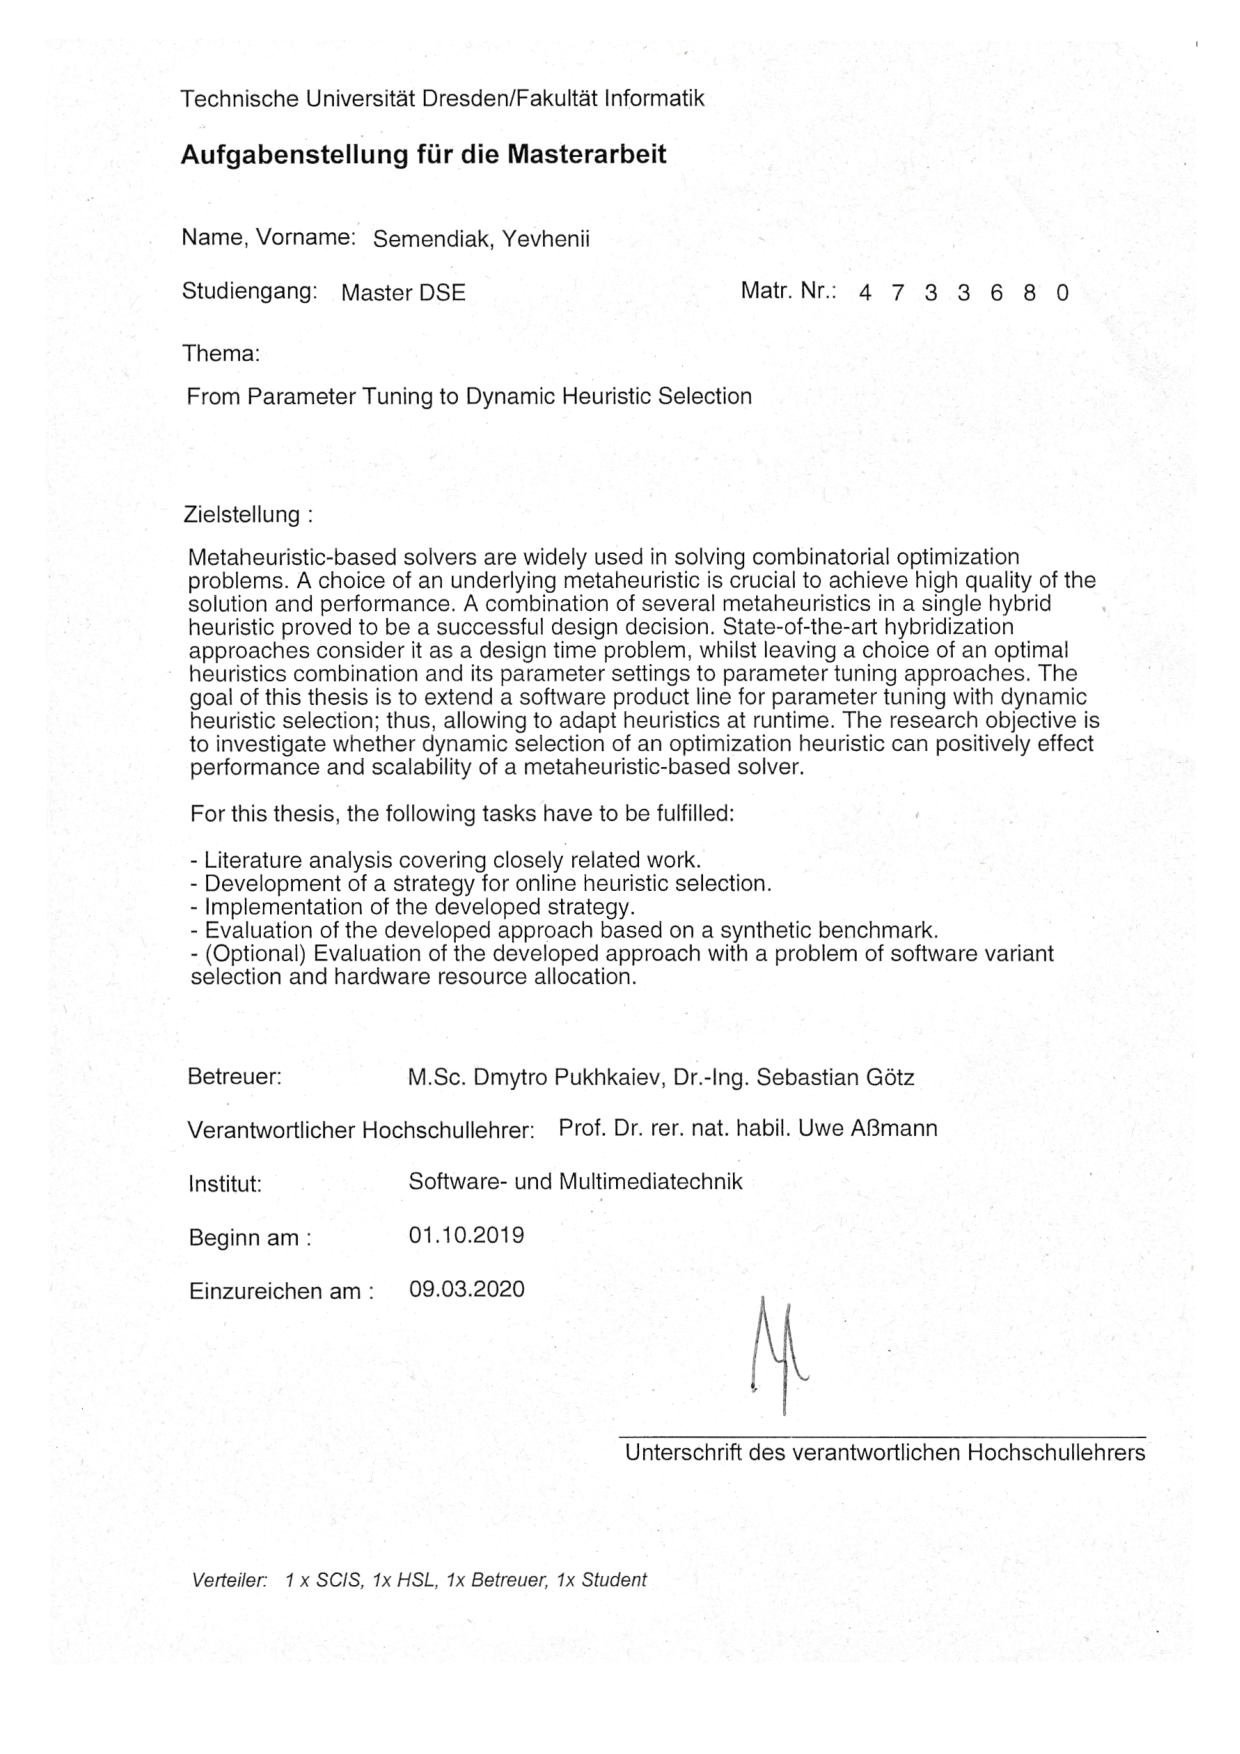
\includepdf{static/taskDescription.pdf}

  \tableofcontents

  \listoffigures
  \listoftables
  
  \newpage
\section*{Abstract}
The importance of balance between exploration and exploitation plays a crucial role while solving combinatorial optimization problems. This balance is reached by two general techniques: by using an appropriate problem solver and by setting its proper parameters. Both problems were widely studied in the past and the research process continues up until now. The latest studies in the field of automated machine learning propose merging both problems, solving them at design time and later strengthening the results at runtime. To the best of our knowledge, the \emph{generalized} approach for solving the parameter setting problem in heuristic solvers has not yet been proposed. Therefore, the concept of merging heuristic selection and parameter control has not been introduced.

In this thesis we propose an approach for generic parameter control in meta-heuristics by means of reinforcement learning (RL). Making a step further, we suggest a technique for merging the heuristic selection and parameter control problems and solving them at runtime using RL-based hyper-heuristic. The evaluation of the proposed parameter control technique on a symmetric traveling salesman problem (TSP) revealed its applicability by reaching the performance of tuned in offline and used in isolation underlying meta-heuristic. Our approach provides the results on par with the best underlying heuristics with tuned parameters.
  \chapter{Introduction}\label{intro}

\section{Motivation}
Heuristic-based optimization is a popular research area~\cite{junger2003combinatorial,biegler2004retrospective,festa2014brief}. Numbers of optimization problems are defined, but an ideal approach for their struggling does not exist. This issue was formalized by the \emph{no-free-lunch theorem for optimization} (NFLT)~\cite{wolpert1997no}, which states that ``all search algorithms have the same average performance over all possible optimization problems''. Heuristic solver acts by means of \emph{exploration} (effort diversification over a search space) and \emph{exploitation} (effort intensification on a promising area) operations. The success of heuristic on the problem at hand is defined by the exposed strength of both operations (E\&E) and the provided balance between them (EvE).

Firstly, one could try to set proper values of hyper-parameters, exposed by the algorithm. This process is formalized under the notion of \emph{parameter settings problem} (PSP), whose resolution can be done before running the algorithm (design time), or while it solves the OP (runtime). The former approach is also called \emph{parameter tuning} and can be tackled by numerous universal tuning systems ~\cite{hutter2009paramils,hutter2011sequential,lopez2016irace,falkner2018bohb,brise2spl}. A key assumption of this software is an expensiveness of the target system evaluation in terms of computational resources. Expensiveness is tackled creating a surrogate learning model, which simulates direct evaluations. The latter approach \emph{parameter control} was originally introduced for evolutionary algorithms~\cite{karafotias2014parameter} and nowadays appears in an \emph{algorithm-dependent} manner. However, even a proper parameter setting may not lead to the best results for the problem at hand. 

The second way for reaching the EvE balance is a proper algorithm selection. It resolves the direct consequence of NFLT by searching appropriate solver for problem at hand and was formalized as the \emph{algorithm selection problem} (ASP). Hyper-heuristics are commonly used for solving ASPs. They may perform low-level heuristic selection before solving the actual problem, or at runtime~\cite{burke2019classification}. To operate on-line, hyper-heuristics often utilize reinforcement learning (RL) techniques~\cite{moriarty1999evolutionary,mcclymont2011markov}, while for design time, a regular parameter tuning could be used.

The research is not at a standstill and nowadays the researchers are actively attempting to merge ASP and PSP into the united \emph{algorithm selection and parameter setting problem} (APSP). For instance, in automatic machine learning such combination was formalized as the \emph{combined algorithm selection and hyper-parameter optimization} problem (CASH)~\cite{thornton2013auto}, while for heuristics the explicit studies of APSP merging and solving at runtime were not found. To tackle ML CASH problem several frameworks based on the existing parameter tuning systems were created~\cite{thornton2013auto,feurer2015efficient,olson2019tpot}. However, those solutions are not applicable in case of heuristics, since they are (1) purely related to ML field and (2) acting at design time due to ML techniques nature. One may follow the ML approach of the united APSP search space definition and solving for heuristics, but it is applicable \emph{only} at design time. However, when it comes to runtime, it turns out that the universal technique for setting the parameters on-line (parameter control) in heuristics has not yet been proposed. It is essential, since this (PSP) is one of two required methodologies for solving heuristic APSP at runtime. The other building block (ASP) is already available in on-line hyper-heuristics.

\section{Research objective}\label{intro: research objective}
The goal of this thesis is to basing on the existing parameter tuning software, propose an \emph{on-line} approach for solving \emph{both} PSP and ASP problems for heuristic solvers.

In order to fulfill the goal defined above, the following \textbf{research questions} should be answered:
\begin{itemize}
	\item \textbf{RQ1} Is it possible to perform the algorithm configuration at runtime on a generic level?
	
	\item \textbf{RQ2} Is it possible to simultaneously perform algorithm selection and parameters adaptation while solving an optimization problem?
	
	\item \textbf{RQ3} What is the effect of selecting and adapting algorithm while solving an optimization problem?
\end{itemize}


\section{Solution overview}
In this thesis we propose the unification of both ASP and PSP into a single problem. In order to do so, we firstly introduce a generic runtime PSP solution; secondly, we suggest joining several PSPs search spaces into a united APSP.

To overcome the sparseness issue we propose a complex solution, which is spread in both search space structure and prediction process. For the APSP representation we suggest using of a data structure, similar to feature trees from software product lines field. Doing so we treat a solver type and its hyper-parameters uniformly as a regular parameter in a search space. The dependencies between parameters are explicitly handled in form of a parent-child relationship. As a result, the search space could be viewed as a layered structure, where on the first level remains (categorical) parameter defining the algorithm type, and on the level(s) below its respective hyper-parameters (categorical and numerical). The prediction process is made sequentially for each level, utilizing the available performance evidences in form of already tried configurations in this optimization session. Therefore, in the united APSP we firstly build a surrogate model for the algorithm type prediction. Afterwards, when the solver type is selected, we filter the performance evidences to operate on data, which is relevant to the selected algorithm type. With this filtered data we build a surrogate for the second level and predict the selected algorithm parameters. Dependencies among algorithm-related parameters are also treated in form of the parent-child relationship, therefore, we proceed the level-wise prediction process until obtaining a completed configuration. Next, we continue solving the underlying OP with the defined algorithm type and its parameters to obtain new evidence and repeat configuration prediction process. This reinforcement learning techniques enables us to solve the APSP on-line, while iteratively tackling the OP at hand. 

The structure of this thesis is organized as follows. Firstly, in \cref{bg} we refresh the reader's background knowledge in the field of optimization problems and solver types, focusing on heuristics. We also review the parameter setting and the available solutions for this problem. In \cref{Concept description} one will find a description of the proposed approach for generic parameter control and APSP problem unification. There we also present both structural and functional requirements for system components. \cref{impl} is dedicated to the review of implementation details, including a code basis selection, aforementioned requirements realization and the developed system workflow representation. We evaluate the proposed concept and discuss the results in \cref{eval}. \cref{conclusion} concludes the thesis and \cref{future work} describes the future work.

  \chapter{Background and Related Work Analysis}\label{bg}
In this Chapter we provide the reader with a review of the basic knowledge in fields of optimization problems and approaches for solving them.
A reader, experienced in field of optimization and search problems, may consider this chapter as an obvious discussion of well-known facts. 
If such notions as a \textit{parameter tuning} and a \textit{parameter control} are not familiar to you or seem the same, we highly encourage you to spend some time reading this chapter carefully.
In any case, it is worth for everyone to refresh the knowledge with a coarse-grained description of topics, mentioned in this section and examine the examples of hyper-heuristics in \cref{bg: hh examples} and systems for parameter tuning in \cref{bg: parameter tuning expamples}.

The structure of this Chapter is defined as follows. Firstly, we give an informal definition of an optimization problem and enumerate possible solver types in \cref{bg:section problems and solvers}. Secondly, we pay attention to the heuristic solvers, their weak points and \emph{No Free Lunch Theorem} in \cref{bg: section heuristics}. Afterwards, in \cref{bg: section Parameters Setting} we discuss the influence of parameter setting and possible approaches to set the parameters. \cref{bg: section cash}, dedicated to \emph{Combined Algorithm Selection and Hyper-parameter Tuning} problem, is followed by conclusion on the literature analysis outlining the thesis' scope in \cref{bg: conclusion}.

\section{Optimization Problems and their Solvers}\label{bg:section problems and solvers}
Our life is full of different difficult and sometimes contradicting choices. Optimization is an art of making good decisions.

A decision between working hard or going home earlier, to buy cheaper goods or to follow brands, to isolate ourselves or to visit friends during the quarantine, to spend more time on a trip planning or to start it instantly. Each decision that we make, has its consequences.

\cref{bg:pic:Optimization tradeoff} outlines the trade-off between decision quality and an amount of effort spent. The underlying idea of the research in optimization is to squash this curve simultaneously down and to the left, therefore, deriving a better result with less cost when solving the optimization problem.

\svgpath{{graphics/Background/}}
\begin{figure}
	\centering
	\includesvg[width=0.7\textwidth]{optimization_concept}
	\caption{Optimization trade-off.}
	\label{bg:pic:Optimization tradeoff}
\end{figure}

\subsection{Optimization Problems}\label{BG: subsection OPs}
While the \emph{search problem} (SP) defines the process of finding a possible solution for the \emph{computation problem}, the \emph{optimization problem} (OP) defined as a special case of the SP, focused on the process of finding the \emph{best possible} solution for computation problem~\cite{goldreich2010p}.

The focus of this thesis is the optimization problems.

Most studies conducted in this field have tried to formalize the OP concept, but the underlying notion is so vast that it is hard to exclude the application domain from the definition. The description of every possible optimization problem and all approaches to its solving are not in the scope of this thesis, while we consider it necessary to present a coarse-grained review in order to make sure that readers are familiar with all the terms and notions mentioned in the thesis. 

To begin with, let us define the optimization \emph{subject}. Analytically, it could be represented as the function $Y = f(X)$ that accepts some input $X$ and reacts to it, providing an output $Y$. Informally, it could be imagined as the \emph{target system} $f$ (TS), shown in \cref{bg:pic:Target System}. It accepts the input information with its \emph{inputs} $X_n$, which are sometimes called variables or parameters, processes them performing some \emph{task} and produces the result on its \emph{outputs} $Y_m$.

\begin{figure}[!h]
	\centering
	\includesvg[width=0.5\textwidth]{TargetSystem}
	\caption{Optimization Target System.}
	\label{bg:pic:Target System}
\end{figure}

Each (unique) pair of sets $X_n^i$ and respective $Y_m^i$ form the $Solution^i$ for computational problem.
All possible inputs $X^i$, where $i=1...N$ form the \emph{search space} of $N$ size, while all outcomes $Y^i$, where $i=1...M$ form an \emph{objective space} of $M$ size.

The solution is characterized by the \emph{objective value(s)} — a quantitative measure of TS performance that we want to minimize or maximize in the optimization problems. We could obtain those value(s) directly, by reading the output on $Y_m$, or indirectly, for instance, noting the wall clock time TS took to produce the output $Y^i$ for given~$X^i$. The solution objective value(s) form the \emph{object} of optimization. 
For the sake of simplicity we here use $Y_m$, \textit{outputs} or \textit{objectives} interchangeably as well as $X_n$, \textit{variables} or \textit{parameters}.

Next, let us highlight the target system characteristics. In works~\cite{biegler2004retrospective,figueira2014hybrid,deb2014multi,amaran2016simulation} dedicated to solving the OPs, the authors distinguished OP characteristics that overlap through each of these works. Among them, we found the following properties to be the most important ones:
\begin{itemize}
	\item \textbf{Input data type} of $X_m$ is a crucial characteristic. All input variables could be (1) \emph{discrete}, where representatives are binary strings, integer-ordered, or categorical data, (2) \emph{continuous}, where variables are usually a range of real numbers, or (3) \emph{mixed}, as the mixture of the previous two cases.

	\item \textbf{Constraints} describe the relationships among inputs and explain the dependencies in allowable values for them. As an example, imagine that having $X_n$ equal to $value$ implies that $X_{n + k}$ should not appear at all, or could take only some subset of all possible values.
	
	\item \textbf{Type of target system} is an amount of exposed knowledge about the dependencies $X \rightarrow Y$ before the optimization process starts. Taking this into consideration, an optimization could be of several types: \emph{white-box} — it is possible to derive the algebraic model of TS, \emph{gray-box} — the amount of exposed knowledge is significant but not enough to build the algebraic model and \emph{black-box} — the exposed knowledge is mostly negligible.
	%In this case the Derivative Free Optimization approaches (such as Surrogate Optimization, different Meta-|Hybrid-|Hyper-Heuristics)  are applicable.
	% http://downloads.hindawi.com/journals/mpe/2015/647234.pdf

	%\paragraph{Dependency types} could be  The inputs to outputs dependencies the of Target System could also be distinguished form perspective of linearity \cite{biegler2004retrospective,figueira2014hybrid}.
	%\textit{Linear dependencies} reveal the Linear Programming Optimization approaches, while with \textbf{Nonlinear dependencies} one should consider Nonlinear Programming.

	\item \textbf{Determinism of TS} is one of the possible challenges, when the output is uncertain. TS is \emph{deterministic}, when in each time it provides an equal output for the same input. However, in most real-life challenges engineers tackle \emph{stochastic} systems, the output of which is affected by random processes happened inside TS.

	\item \textbf{Cost of evaluation} is an amount of resources (energy, time, money, etc.) TS should spend to produce the output for particular input. It varies from \emph{cheap}, when TS could be an algebraic formula and task evaluation is a simple mathematic computation, to \emph{expensive}, when the TS is a pharmaceutical company, and the task is to perform a whole bunch of tests for a new drug, which may last years. 

	\item \textbf{Number of objectives} is a size of the output vector $Y_m^i$. With regard to this, the optimization could be either single- ($m=1$), or multi- ($m=2...M$) objective, where the result is one single solution, or a set of non-dominated (Pareto-optimal) solutions.
\end{itemize}

Most optimization problem types could be obtained by combining different types of each characteristic listed above.

In this thesis we tackle practical combinatorial problems, where the most prominent examples are \emph{bin packing}~\cite{martello1990bin}, \emph{job-shop scheduling}~\cite{blazewicz1996job} or \emph{vehicle routing}~\cite{toth2002vehicle} optimization problems.
All combinatorial problems are \emph{NP-Complete} meaning they are in both \emph{NP} and \emph{NP-Hard} complexity classes~\cite{garey1979computers}. NP complexity implies that the solution is verifiable in the polynomial time, while in the NP-Hard case the problem can be transformed into other NP-Complete problem in polynomial time, allowing to use a different solving algorithm.

As an example, let us grasp these characteristics for \emph{traveling salesman problem} (TSP)~\cite{applegate2006traveling} — an instance of the vehicle routing problem~\cite{laporte1992vehicle} and one of the most frequently studied a combinatorial OP (here we consider deterministic and symmetric TSP).
The informal definition of TSP is as follows: ``Given a set of $N$ cities and the distances between each of them, what is the shortest path that visits each city once and returns to the origin city?''
With respect to our previous definition of the optimization problem, the target system here is a function that evaluates the length of proposed path. The TSP distance (or cost) matrix is used in this function for the evaluation and it is clear that this TS exposes all internal knowledge therefore, it is a white box.
The input $X_n$ is a vector of city indexes as a result, the type of input data is non-negative integers. There are two constraints for the path: it should contain only unique indexes (visit each city only once) and it should start and end from the same city:~$[2 \rightarrow 1 \rightarrow ... \rightarrow 2]$.
Since the cost matrix is fixed and not changing during the solving process, the TS is considered to be deterministic and costs of two identical paths are always the same. Nevertheless, there exist Dynamic TSP where the cost matrix changes at runtime to reflect more realistic real-time traffic updates~\cite{cheong2011dynamic}.
It is cheap to compute a cost for a given path using the cost matrix therefore, overall solution evaluation in this OP is cheap, and $n = N!$ is the overall number of solutions. Since we are optimizing only the route distance, this is a single-objective OP.


\subsection{Optimization Problem Solvers}\label{BG: subsection OP Solvers}
Most of the optimization problems could be solved by an \emph{exhaustive search} — trying all possible combinations of the input variables and choosing the one, which provides the best objective value. This approach guarantees to find a globally optimal solution of the OP. But when the search space size significantly increases, the brute-force approach becomes infeasible and in many cases solving even the relatively small problem instances take too much time.

Here, different optimization techniques come into play. Characteristics exposed by target system could restrict and sometimes strictly define the applicable approach.
For instance, imagine you have a white-box deterministic TS with a discrete constrained input data and cheap evaluation. The OP in this case could be solved using the \emph{Integer Linear Programming} (ILP), or a heuristic approaches. But if this TS turned out to be a black-box, the ILP approaches will not be applicable anymore and one should consider using the heuristics~\cite{biegler2004retrospective}.

Evidently, there exist a lot of different facets for optimization problem solvers classification, but they are a subject of many surveying works~\cite{junger2003combinatorial,biegler2004retrospective,festa2014brief}. In this thesis, as the point of interest we highlight only two of them.

\begin{itemize}
	\item \textbf{Solution quality} perspective:
	\begin{enumerate}
		\item \textbf{Exact} solvers are those algorithms that always provide an optimal OP solution.
		\item \textbf{Approximate} solvers produce a sub-optimal output with guarantee in quality (some order of distance to the optimal solution).
		\item \textbf{Heuristics} solvers do not give any worst-case guarantee for the final result quality.
	\end{enumerate}
	
	\item \textbf{Solution availability} perspective:
	\begin{enumerate}
		\item \textbf{Completion} algorithms report the results only at the end of their run.
		\item \textbf{Anytime} algorithms are designed for stepwise solution improvement thus, could expose intermediate results.
	\end{enumerate}
\end{itemize}

Each of these algorithm characteristics provides their own advantages, having, however, their own disadvantages. For instance, if solution is not available at any time, one will not be able to control the optimization process. On the contrary, if it is available, the overall performance may decrease. 
If the latter features are more or less self-explanatory, the former require more detailed explanation.

\subsubsection{Solution Quality}
\paragraph{Exact Solvers.}
As was stated above, the exact algorithms are those, which always solve OP to guaranteed optimality. For some OP it is possible to develop an effective algorithm that is much faster than the exhaustive search — they run in a super-polynomial time, instead of exponential, still providing an optimal solution. As authors claimed in~\cite{woeginger2003exact}, if the common belief $P \ne NP$ is true, the super-polynomial time algorithms are the best we can hope to get when dealing with the NP-complete combinatorial problems.

According to the definition in~\cite{fomin2013exact}, the objective of an exact algorithm is to perform much better (in terms of running time) than the exhaustive search. In both works~\cite{woeginger2003exact,fomin2013exact} the authors enumerated main techniques for designing the exact algorithms. Each of these techniques contributes to this `better' independently and later they could be combined.

You may find a brief explanation of them below:
\begin{itemize}
	\item \textbf{Branching and bounding} techniques, when applied to the original problem, split the search space of all possible solutions (e.g. exhaustive enumeration) to a set of smaller sub-spaces. More formally, this process is called \emph{branching the search tree into sub-trees}. This is done with an intent to prove that some of sub-spaces never lead to an optimal solution and thus could be rejected.
	
	\item \textbf{Dynamic programming across sub-sets} technique could be combined with the  branching techniques. After forming the sub-trees, the dynamic programming attempts to derive the solutions for the smaller subsets and later combine them into the solutions for the lager subsets. This process repeats until the solution for original search space obtained.
	
	\item \textbf{Problem preprocessing} could be applied as an initial phase of the solving process. This technique is dependable upon the underlying OP, but when applied properly, it significantly reduces the running time. A simple example from~\cite{woeginger2003exact} elegantly illustrates this technique: imagine a problem of finding a pair of two integers $x_i$ and $y_i$ in $X_k$ and $Y_k$ sets of unique numbers ($k$ here denotes the size of sets) that sum up to an integer $S$. The exhaustive search approach implies enumerating all $x-y$ pairs. The time complexity in this case is $O(k^2)$. But if at first we consider the data preprocessing by sorting and afterwards, using the bisection search repeatedly in these sorted arrays to find $k$ values $S - y_i$, then the overall time complexity reduces to $O(k\log(k))$.
\end{itemize}

\paragraph{Approximate Solvers.} When the OP cannot be solved to optimal in polynomial time, the only solution is to start thinking of the alternative ways to tackle it. A common decision is to apply the requirement \emph{relaxation techniques}~\cite{roubivcek2011relaxation} to derive the approximated solution.
Approximate algorithms are representatives of the theoretical computer science. They were created in order to tackle the computationally difficult (not solvable in super-polynomial time) white-box OP. Words of Garey and Johnson (computer scientists, authors of \textit{Computers and Intractability} book~\cite{garey1979computers}) could pay a perfect description of such approaches: ``I can't find an efficient algorithm, but neither can all of these famous people.''
%If the widely believed conjecture $P \ne NP$ is true, a wide range of OPs (ILP) are $NP-hard$ and cannot be solved with exact solvers in polynomial time, thus require relaxation either in efficiency or quality of optimization.

Unlike exact, approximate algorithms relax the quality requirements and solve the OP effectively with the provable assurances on the result distance from an optimal solution~\cite{williamson2011design}. The worst-case results quality guarantee is crucial in the approximation algorithms design and involves the mathematical proofs.

How do these algorithms guarantee on quality, if the optimal solution is unknown beforehand? — a reasonable question arises at this point. Certainly, it sounds contradictory, but the comprehensive answer to this question requires an explanation of the key approximation algorithms design techniques that is not in the scope of this thesis. Nevertheless, let us briefly describe these techniques.

In~\cite{williamson2011design} the authors provided several techniques to approximate solvers' design. For instance, the \emph{Linear Programming} (LP) relaxation plays a central role in approximate solvers. It is well known that solving the ILP is \textit{NP-hard} problem. However, it could be relaxed to the polynomial-time solvable linear programming. %Those, one of techniques is relaxation of ILP to LP. An optimal solution for LP will have value $S_LP \le S_IP = OPT$ (for the minimization case). Here we could derive a lower bound for the original minimization or upper bound for maximization problem. 
Later, a fractional solution for the LP will be rounded to obtain a feasible solution for the ILP. % that is within a cerain factor $f$ the value of the LP $S_LP$. Thus, the ILP solution will cost no more than $f * OPT$.
Different rounding strategies define separate approximate solver techniques~\cite{williamson2011design}: 
\begin{itemize}
	\item \textbf{Deterministic rounding} follows a predefined strategy.
	\item \textbf{Randomized rounding} performs a round-up of each fractional solution value to the integer uniformly.
\end{itemize}

In contrast to rounding, another technique requires building a \emph{Dual Linear Program} (DLP) for a given linear program. This approach utilizes the \emph{weak} and \emph{strong duality} properties of DLP to derive the distance of the LP solution to the original ILP optimal solution. Other properties of DLP form a basis for the \emph{Primal-dual} algorithms. They start with a dual feasible solution and use the dual information to derive the primal linear program solution (possibly infeasible). If the primal solution is not feasible, the algorithm modifies the dual solution increasing the dual objective function values. In any case, these approaches are far beyond the thesis scope, but in case of an interest reader could start his own investigation from~\cite{williamson2011design}. 

\paragraph{Heuristics.} As opposed to the solvers mentioned above, heuristics do not provide any guarantee on the solution quality. They are applicable not only to the white-box TS but also to the black-box cases. These approaches are sufficient to quickly reach an immediate, short-term goal in such cases, when finding an optimal solution is impossible or impractical because of the huge search space size.

As in the reviewed above approaches, here exist many facets for classification.
We start from the largest one, namely the \textit{level of generality}:
\begin{itemize}
	\item \textbf{Simple heuristics} are the specifically designed to tackle the concrete problem algorithms. They fully rely on the domain knowledge, obtained from the optimization problem. Simple heuristics do not provide any mechanisms to escape a local optimum therefore, could be easily trapped to it~\cite{pearl1984intelligent}.
	
	\item \textbf{Meta-heuristics} are the high-level heuristics that being domain knowledge-dependent, also provide some level of generality to control the search. They could be applied to broader range of the OPs. They are often nature-inspired and comprise mechanisms to escape the local optima but may converge slower than the simple heuristics. For the more detailed explanation we refer to survey~\cite{bianchi2009survey}.
	
	\item \textbf{Hybrid-heuristics} arise as the combinations of two or more meta-heuristics. They could be imagined as the recipes merge from the cookbook, combining the best decisions to create something new and presumably better.
	
	\item \textbf{Hyper-heuristics} are the algorithms that operate in the search space of \emph{low-level heuristics} (LLH). Instead of tackling the original problem, they choose (or construct) LLHs, which will tackle this problem for them~\cite{burke2003hyper}. 
\end{itemize}

In the upcoming \cref{bg: section heuristics}, dedicated to heuristics, we provide more detailed information on each of the approaches mentioned above.


\subsubsection{The Most Suitable Solver Type}
\epigraph{``Fast, Cheap or Good? Choose two.''}{\textit{The old engineering slogan.}}

At this point, we have reached the crossroads and should make a decision, which way to follow.

Firstly, we have the exact solvers for the optimization problems. As mentioned above, they always guarantee to derive an optimal solution. Today, tomorrow, maybe in the next century, but eventually the exact solver will find it. The only thing we need is to construct the exact algorithm. This approach definitely offers the best final solution quality however, it sacrifices the solver construction simplicity and the speed in problem-solving.

Secondly, we have the approximate solvers. They do not guarantee to find the one and only optimal solution but suggest a provably good instead. From our perspective, the required effort for constructing the algorithm and proving its preciseness remains the same as for the exact solvers. However, this approach outperforms the previous one in the speed of problem-solving, sacrificing a reasonably small amount of the result quality. It sounds like a good deal.

Finally, the remaining heuristic approaches. They quickly produce a solution, in comparison to the previous two. In addition, they are much easier to apply for the specific problem — there is no need to build complex mathematical models or prove the theorems. However, the biggest flaw in these approaches is the absence of the solution quality guarantee.

As we mentioned in \cref{BG: subsection OPs}, this thesis is dedicated to facing the practical combinatorial problems, such as the TSP. They are NP-complete, that is why we are not allowed to apply the exact solvers. In both approximate and heuristic solvers we are sacrificing the solution quality, though in different quantities. Nevertheless, the heuristic algorithms repay in the development time and provide the first results faster. The modern world is highly dynamic, in the business survive those, who are faster and stronger. In the most cases, former plays the crucial role for success. The great products are built iteratively, enhancing existing results step-by-step and leaving the unlucky decisions behind. It motivates us stick to the heuristic approach within the scope of the thesis.

In the following \cref{bg: section heuristics} we shortly survey different heuristic types and examples. We analyze their properties, weaknesses and ways to deal with them. As the result, we select the best-suited class of heuristics for solving the TSP problem.

\section{Heuristic Solvers for Optimization Problems}\label{bg: section heuristics}
We base our descriptions of heuristics and their examples on the mentioned in \cref{BG: subsection OPs} traveling salesman problem. The input data $X$ to our heuristics will be the problem description in form of a distance matrix (or coordinates to build this matrix), while as an output $Y$ from heuristics we expect to obtain the sequence of cities, depicting the route plan.

% In general, when a heuristic applied to particular problem do not use the gradient or Hessian matrix of the objective function for optimizations \cite{boussaid2013survey}.

Most heuristic approaches utilize the following concepts:
\begin{itemize}
	\item \textbf{Neighborhood}, which defines a set of solutions that could be derived performing a single step of the heuristic search.
	\item \textbf{Iteration}, which could be defined as an action (or a set of actions) performed over the solution in order to derive a new, hopefully better one.
	\item \textbf{Exploration} (diversification), which is the process of discovering previously unvisited and presumably high-quality parts of the search space.
	\item \textbf{Exploitation} (intensification), which is the usage of already accumulated knowledge (solutions) to derive a new solution but similar to existing one.
\end{itemize}

%Naturally, there are lots of characteristics that could be used to classify heuristics starting from the use of memory, kind of neighborhood, way to derive a solution (construction or perturbation) or number of solutions carried from one iteration to following. 

\subsection{Simple Heuristics}
As we mentioned above, simple heuristics are domain-dependent algorithms, designed to solve a particular problem.
They could be defined as the rules of thumb, or strategies to utilize the information, exposed by the TS and obtained from the previously found solutions, to control the problem-solving process~\cite{pearl1984intelligent}. 

Scientists draw the inspiration for heuristics creation from all aspects of our being: starting from the observations of how humans tackle daily problems using intuition, and proceeding to the mechanisms discovered in nature. The two main types of simple heuristics were outlined in~\cite{burke2019classification}: \textit{constructive} and \textit{perturbative}. 

The first type aggregates the heuristics which construct the solutions from its parts step by step. 
A prominent example of constructive approach is a \textit{greedy algorithm}, which can also be called the \textit{best improvement local search}. When applied to TSP, it tackles the path construction simply accepting the next closest city from currently discovered one. Generally, the greedy algorithm follows the logic of making a sequence of locally optimal decisions therefore, it ends up in a local optimum after constructing the very first solution. 

The second type, called a \textit{local search}, implies heuristics which operate on the complete solutions, perturbing them. A simple example of the local search is a \textit{hill climbing algorithm}, also known as a \textit{first improvement local search}~\cite{voudouris1999guided}. This heuristic accepts a better solution as soon as it finds it, during the neighborhood evaluation. This approach plays a central role in many high-order algorithms however, it could be very inefficient, since in some cases the neighborhood could be enormously huge. 

Indeed, since the optimization result is fully dependent on the starting point. The use of simple local search heuristics might not lead to a globally optimal solution. Nevertheless, in this case the advantage will be the implementation simplicity~\cite{williamson2011design}.

 
\subsection{Meta-Heuristics}\label{bg: mh}
Meta-Heuristic (MH) is an algorithm, created to solve a wider range of complex optimization problems with no need to deeply adapt it to each problem.

The research in MHs field arose even before 1940s, when the MHs were already actively applied. However, there were no all-embracing and complex studies of MHs at that time. The first formal studies appeared between 1940s and 1980s. Deep and profound research in this field reaches its most active stage in the late 1990s, when the numerous MHs popular nowadays were invented. The period from 2000 and up till now the authors in~\cite{sorensen2017history} call the framework growth time, when the meta-heuristics widely appear in form of frameworks, providing a reusable core and requiring only the domain-specific adaptation.

The prefix \emph{meta-} indicates the algorithms to be of the \textit{higher level} when compared to simple problem-dependent heuristics. The static part of the algorithms is stable and problem independent, it forms the core of an algorithm and usually exposes \textit{hyper-parameters}, which could be used for the algorithm configuration. The changeable parts are domain-dependent and should be adapted for problem at hand. Many MHs contain stochastic components, which provide abilities to escape from local optimum. However, it also means that the output of meta-heuristic is non-deterministic and it could not guarantee the result preciseness~\cite{boussaid2013survey}.

The meta-heuristic optimizer success on a given OP depending on the \textit{exploration vs exploitation balance}. If there is a strong bias towards diversification, the solving process could naturally skip a good solution while performing huge steps over the search space, but in case of intensification domination, the process will quickly settle in the local optima. The disadvantage of the simple heuristic approaches mentioned above is a high exploitation dominance, since they simply do not have the components contributing to exploration. In most of the cases, it is possible to decompose MH into simple components and clarify, to which of competing processes contributes each component. Often, the simple heuristics are used as the intensification component.

In general, the difference between existing meta-heuristics lays in a particular way how they are trying to achieve this balance, but the common characteristic is that the most of them are inspired by real-world processes — physics~\cite{van1987simulated}, biology~\cite{sastry2005genetic}, ethology~\cite{teodorovic2006bee,dorigo2007ant,salcedo2014coral}, and even evolution~\cite{beyer2002evolution,eiben2015evolutionary}.


\subsubsection{Meta-Heuristics Classification}
When the creation of novel methodologies has slowed down, the research community began to organize and classify the created algorithms.

\begin{figure}[!b]
	\centering
	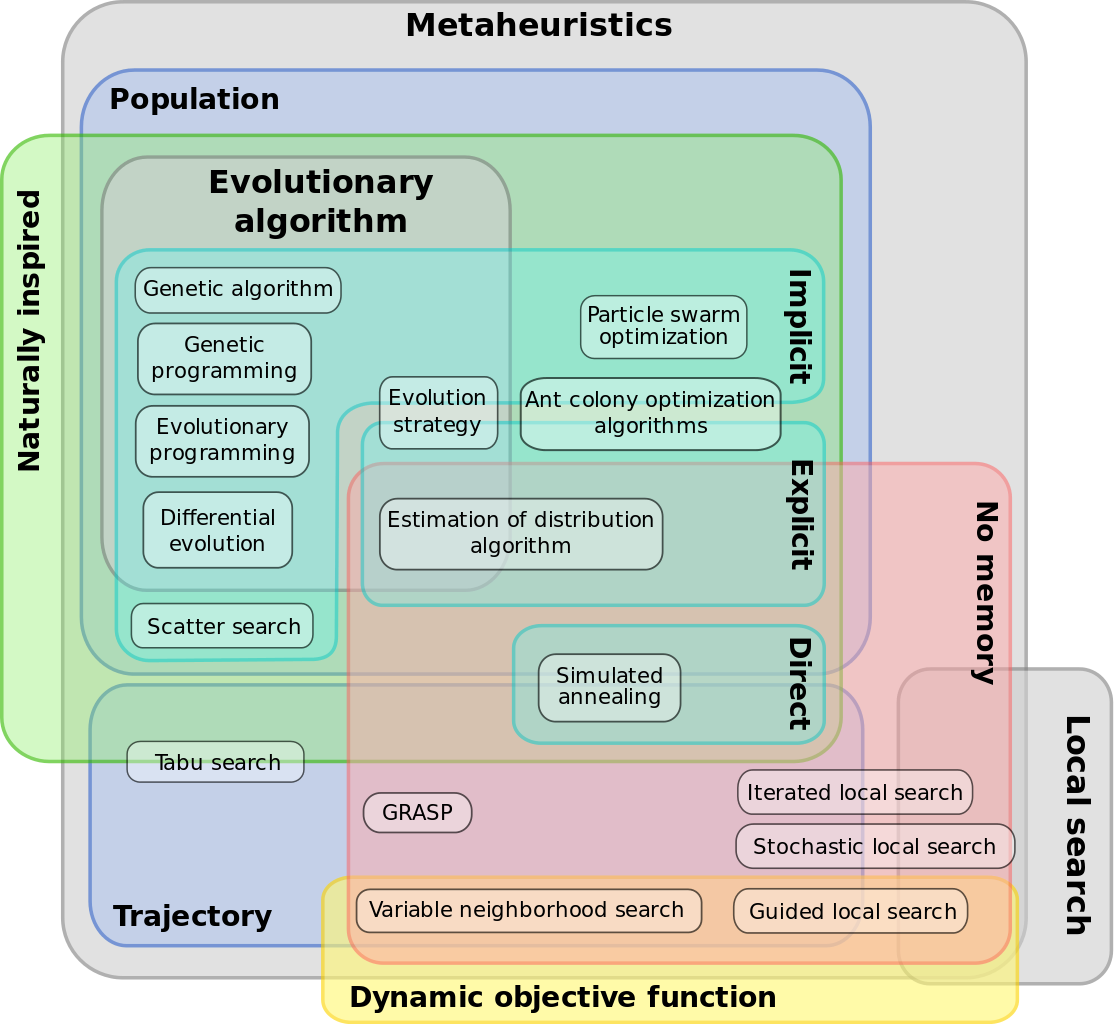
\includegraphics[width=0.7\textwidth]{graphics/Background/Metaheuristics_classification}
	\caption{Meta-heuristics Classification~\cite{dreo2007dreaming}.}
	\label{BG: MH classification}
\end{figure}

As an example, \cite{birattari2001classification} highlights the following classification facets:
\begin{itemize}
	\item The \textbf{walk-through search space method} could be either trajectory-based or discontinuous. The first one corresponds to a closed walk through the neighborhood where such prominent examples as \textit{iterated local search}~\cite{lourencco2003iterated} or \textit{tabu search}~\cite{glover1989tabu} do exist. The second one allows large jumps in the search space, where the examples are such MHs as \textit{variable neighborhood search}~\cite{hansen2003variable} or \textit{simulated annealing}~\cite{kirkpatrick1983optimization}.
	
	\item The \textbf{number of concurrent solutions} could be either single or multiple. Such approaches as tabu search, simulated annealing or iterated local search are examples of algorithms with a single concurrent solution. Evolutionary algorithms~\cite{eiben2015evolutionary}, ant colony optimization~\cite{dorigo2007ant} or particle swarm optimization~\cite{kennedy1995particle} are the instances of algorithms with multiple concurrent solutions (the population of solutions).
	
	\item From the \textbf{memory usage} perspective, we distinguish those approaches which do and do not utilize the memory. Tabu search explicitly uses memory in form of tabu lists to guide the search, but simulated annealing is memory-less.
	
	\item The \textbf{neighborhood structure} could be either static or dynamic. Most local search algorithms, such as simulated annealing and tabu search are based on a static neighborhood. Variable neighborhood search is an opposite case, where various structures of neighborhood are defined and interchanged while the algorithm solves the OP.
\end{itemize}

There are many more classification facets, which are not in the scope of this thesis. \cref{BG: MH classification} illustrates the summarized classification including some characteristics and well-known meta-heuristic instances we did not mention.


\subsubsection{Meta-Heuristics Examples}\label{BG: MH Examples}
At this point, let us briefly describe some of the most prominent and widely used meta-heuristics. It is motivated by the later usage of them in our approach, described in \cref{impl: LLH}.

\paragraph{Evolutionary Algorithms (EAs)} are directly inspired by the processes in nature, described in evolution theory. The common underlying idea in all of these methods is as follows: if we put a population of individuals (solutions) into an environment with limited resources (population size limit), a competition processes cause natural selection, where only the best individuals survive~\cite{eiben2015evolutionary}.

Three basic actions are defined as operators of EAs: a \emph{recombination} operator selects the parent solutions, which later will be combined to produce the new ones (offspring); a \emph{mutation} operator, when applied to solution, creates a new and very similar one. Applying both operators,the algorithm creates a set of new solutions — the offspring, whose quality is then evaluated with the TS. After that, a \textit{selection} operator is applied to all available solutions (parents and offspring) to keep the population size within the defined boundaries. This process is repeated, until some termination criterion is fulfilled. For instance, the maximal iterations counter was reached, the number of TS evaluations exceeds the defined maximal value, or the solution with the required quality is found. The high-level work-flow of EA is depicted in \cref{bg:pic:EAs}.

\begin{figure}
	\centering
	\includesvg{EA}
	\caption{Evolutionary Algorithms Workflow.}
	\label{bg:pic:EAs}
\end{figure}

The well-known examples of EAs include the \textit{genetic algorithm}~\cite{sastry2005genetic}, \textit{genetic/evolutionary programming}~\cite{koza1992evolution}, \textit{evolution strategies}~\cite{beyer2002evolution}, and many other algorithms.

\emph{Genetic Algorithm} (GA) is the first of all associated with the Evolutionary Algorithms. GA traditionally has a fixed workflow: given an initial population of $\mu$ usually randomly sampled individuals, the parent selection operator creates pairs of parents, where the probability of each solution to become a parent depends on its objective value (fitness, or results). After that, the crossover operator is applied to every created pair with a probability $p_c$ and produces children. Then, newly created solutions undergo the mutation operator with an independent probability $p_m$. The resulting offspring perform a tournament within the selection operator and $\mu$ survivals replace the current population~\cite{eiben2015popular}. Distinguishable characteristic of vanilla GA is the usage of the following operators: bit-string solution representation, one-point crossover recombination, bit-flip mutation and generational selection (only children survive).

\emph{Evolution Strategy} (ES), comparing to GA, is working in a vector space of the solution representation. However, they also use the population size of $\mu$ individuals and $\lambda$ offspring generated in each iteration. While the general workflow for all EAs remains the same, they mostly differ in underlying operators. In ES, the parent selection operator takes a whole population into consideration uniformly, the recombination scheme could involve more than two parents to create one child. To construct a child, the recombination operator joins parents alleles in two possible ways: (1) with uniform probability for each parent (discrete recombination), or (2) averaging the weights of alleles by parent solution quality (intermediate recombination). There are two selection schemes, used in such algorithms. $(\mu,\lambda)$: discard all parents and select only among offspring highly enriching the exploration, and $(\mu+\lambda)$: include also the predecessor solutions into selection, which is often called the \textit{elitist selection}~\cite{eiben2015popular}. In many cases, the ES utilizes a very useful feature of \emph{self-adaptation}: changing the mutation step sizes at runtime, which we will discuss in \cref{bg: parameter control}.

\paragraph{Simulated Annealing (SA).} This is the other type of meta-heuristics, inspired by the technique used in metallurgy to obtain `well-ordered' solid-state of metal~\cite{van1987simulated}. An annealing technique imposes a globally minimal internal energy state and avoids locally minimal semi-stable structures. 

The SA treats the search process as a metal with a high temperature at the beginning and lowering it to the minimum while approaching the end. %SA algorithm handles the optimization objective as annealing threat the material energy. 
It starts with an initial solution $S$ creation (randomly or using some other heuristic) and temperature parameter $T$ initialization. At each iteration, a new solution candidate is sampled within a neighborhood of the current solution: $S^* \leftarrow N(S)$. The newly sampled solution replaces the older one, if (1) optimization objective $f(S^*)$ dominates over $f(S)$ or (2) with a probability that depends on a quality loss and current value of $T$, see \cref{bg: SA acceptance criteria}.

\begin{equation}
p(T, f(S^*), f(S)) = \exp(-\frac{|f(S^*) - f(S)|}{T})
\label{bg: SA acceptance criteria}
\end{equation}

At each iteration the temperature parameter $T$ value is decreased following some type of annealing schedule, which is also called \textit{cooling rate}~\cite{boussaid2013survey}. The weak side here is that the quality of each annealing schedule is the problem-dependent and cannot be determined beforehand. Nevertheless, the SA algorithms with adaptive parameters do exist and address this problem changing the cooling rate or temperature parameter $T$ during the search process. Later, we will shortly review these techniques in \cref{bg: parameter control: SA}.


\subsection{Hybrid-Heuristics}
The hybridization of different systems often provides a positive effect — taking the advantages of one system and merging them with characteristics of the other, getting the best from both systems. The same idea is applicable in the case of meta-heuristics. Imagine you have two algorithms, one is biased towards exploration, the other — towards exploitation. Applying them separately, the expecting results in most cases may be far away from the optimal as the outcome of disrupted diversification-intensification balance. However, when merging them into, for example, repeated stages of hybrid heuristic, one will obtain the advantages of both escaping a local optimum and finding a good quality result. 

Most of the available hybridization algorithms are created with the help of this idea of two heuristics staging combination, one of which is suited for the exploration and other is better for the exploitation.

The methods to construct the hybrids are mostly defined by the underlying heuristics. Therefore, to the best of our knowledge they could not be generalized and classified in an appropriate way. Commonly, there is only one shared characteristic in the usage of a \emph{staging approach}, in which the output of one algorithm is used as the initial state of the other. 

As during the simple heuristics review, here we also introduce examples of performed hybridization in order to provide the reader a better understanding how can be combined different algorithms components and what is the effect on the aforementioned balance.

\subsubsection{Hybrid-Heuristics Examples}
\paragraph{Guided Local Search and Fast Local Search.}
The main focus of guided local search (GLS) in this case, lies in the search space exploration and the process guidance using incubated information. To some extent, the GLS approach is closely related to the frequency-based memory usage in tabu search. During the runtime, GLS modifies the problem cost function to include penalties and passes this modified cost function to the local search procedure. These penalties form a memory that characterizes a local optimum and guide the process out of it. The more time algorithm spends in the local optimum, the higher are the penalties. A local search procedure is carried out by fast local search (FLS) algorithm, where the main advantage is a quick neighborhood traversal. It is done by breaking it up into a number of small sub-neighborhoods. Afterwards, while performing the depth-first search over these sub-neighborhoods, it ignores those, which do not make any improvements. At some point in time, FLS reaches the local optimum and passes back the control in GLS to update the penalties and repeat the iteration~\cite{tsang1997fast}.

\paragraph{Direct Global and Local Search.}
This hybridization consists of two stages: the stochastic global coarse pre-optimization and the deterministic local fine-optimization. At the first stage, the authors apply one of the two abovementioned meta-heuristics --- genetic algorithm or simulated annealing~\cite{hooke1961direct}. A transition from global to local search happens after reaching the predefined conditions. For instance, when the number of TS evaluations exceeds a boundary, or when no distinguishable improvement was made in the last few iterations. Then, the pattern search algorithm also known as the direct, derivative-free, or black-box search performs fine-optimization. The hybrid-heuristic terminates when the pattern search converges to the local optima~\cite{syrjakow1999efficient}.

\paragraph{Simulated Annealing and Local Search.}
After the brief explanation of the previous two hybrids, it is not so difficult to guess, how the next hybridization works.
The authors in their work~\cite{martin1996combining} called this method `Chained Local Optimization'. Therefore, it is yet another representative of staged hybridization.
Iteration starts with the current solution perturbation, called \emph{kick} in~\cite{martin1996combining}, referring to a dramatic change of a current position within the search space. Afterwards, the hill climbing algorithm is applied to intensify the obtained solution. After reaching the local optimum, hill climber passes the control flow back to the simulated annealing for acceptance criteria evaluation, which finishes the iteration.

\paragraph{EMILI.}
Easily Modifiable Iterated Local search Implementation (EMILI) is a framework system for the automatic generation of new hybrid stochastic local search algorithms~\cite{pagnozzi2019automatic}. EMILI is a solver for permutation flow-shop problems (PFSP), also known as flow shop scheduling problems~\cite{reza2005flowshop}. In PFSP the search of an optimal sequence of steps to create products within a workshop is performed.
In this framework, the authors have implemented both generic algorithmic- and problem-specific building blocks. They also have defined grammar-based rules for those blocks composition and used an automatic parameter tuning tool called IRACE~\cite{lopez2016irace} in order to find the high performing algorithm configurations. The workflow of EMILI could be split into three steps: (1) adaptation of the grammar rules to specific PFSP objective representations (makespan, sum completion times and total tardiness), (2) generation of all possible hybrid heuristics for each PFSP representation and (3) execution of IRACE to select the best-performing hybrid for each problem. 

From our perspective, the described approach of automatic algorithm generation is an example of construction hyper-heuristics, which we describe in the upcoming \cref{bg: hh}. However, we are not authorized to change the system class (from hybrid- to hyper-heuristic) defined by the EMILI authors.


\subsection{No Free Lunch Theorem}
At this point, an obvious question may arise: ``If there already exist excellent and well-performing heuristics, is there any need to put an effort into developing new algorithms instead of using existing ones?'' The answer to this question is quite simple — the perfect algorithm suited for \emph{all} OP does not exist and cannot exist at all. 
The empirical research has shown that some meta-heuristics perform better with some types of problems, but are less-performing with others. In addition to that, for different instances of the same problem type, the same algorithm could result in unexpected performance metrics. Moreover, even at different stages of the same problem solving process the dominance of one heuristic over another could change. 

All search algorithms perform exactly the same, when the results are averaged over all possible optimization problems. If an algorithm is gaining the performance in one problem class, it loses in another class. This is a consequence of a so-called \emph{no free lunch theorem for optimization} (NFLT)~\cite{wolpert1997no}.

In fact, one cannot predict, how exactly one or another algorithm will behave with a problem at hand. A possible and most obvious way is to probe one algorithm and compare its performance to another one during the problem-solving process. In this case, simple heuristics and meta-heuristics are out of the competition, since once the optimization problem is solved, one probably would not try to solve it for the second time.
Here, the \emph{hyper-heuristics} come into play to intelligently pick heuristics suitable to the problem at hand. We will proceed with their description outlining the way they deal with the NFLT consequences in the following section.


\subsection{Hyper-Heuristics}\label{bg: hh}
Many of state-of-the-art heuristics and meta-heuristics are developed in a complex and very domain-dependent way, which causes problems with their reuse. It motivated the research community to raise the question of a generality level at which the optimization systems can operate and still provide good quality solutions for various optimization problems. 

The term \textbf{hyper-heuristic} (HH) was defined to describe an approach of using some \textit{high-level-heuristics} (HLH) to select over other \textit{low-level-heuristics} (LLH) and apply them to solve the \textit{class} of optimization problems rather than a particular instance. Indeed, scientists report that the combination of different HLH produces better results when applied separately~\cite{drake2019recent}.
This behavior can be explained by the way of how the search process evolves in time. When one applies a heuristic, it sooner or later converges to some extreme point, hopefully global optimum. But it is `blind' to others, not visited regions of the search space. Changing the trajectory of an investigation by (1) drastically varying the neighborhood, (2) changing the strategy of neighborhood exploration and exploitation could (1) bring one to those previously unreachable zones (2) in more rapid ways. However, usually it is hard to predict how one LLH will behave in every stage of the search process in comparison to another. In hyper-heuristics, this job was encapsulated into the HLH and performed automatically. 

In~\cite{moriarty1999evolutionary} the authors made an infer that HHs can be viewed as a form of reinforcement learning (RL), which is a logical conclusion, especially if rephrased to \textit{hyper-heuristics utilize reinforcement learning methodologies}.

\begin{figure}
	\raggedleft
	\includesvg[width=0.75\textwidth]{HH}
	\caption[Hyper-Heuristics]{Hyper-Heuristics.\footnote{Icons are taken from \url{https://thenounproject.com/}}}
	\label{bg:pic:HH}
\end{figure}

The new concept, which was implicitly used in meta-heuristics, but explicitly pointed out in hyper-heuristics is the \emph{domain barrier} (see \cref{bg:pic:HH}).
As was stated previously, HH do not tackle the OP directly, but use LLH instead. This means that usually HH is minimally aware of the domain details, such as data types, relationships, etc. within a domain. This information is rather encapsulated in LLHs, therefore, HHs could be applied to a broader range of optimization problems.

With this idea, many researchers started to create not only hyper-heuristics to tackle a concrete optimization problem class, but also frameworks with building blocks for their creation.


\subsubsection{Classification}
Although the research in hyper-heuristics field is actively going on, many algorithm instances were already created and some trials to organize approaches were conducted in~\cite{ryser2014review,drake2019recent,burke2019classification,kerschke2019automated}.

Researchers in their surveys classify HHs by different characteristics, some of which overlap, but sometimes important features (from our perspective) were not highlighted in all works. 

In this section we unite of those important hyper-heuristics classification facets in order to better justify the goal of this thesis.

To begin with, there are two broadest classes, which differentiate HH \emph{routine}, also called \emph{nature of high-level-heuristic search space}~\cite{burke2013hyper,burke2019classification,drake2019recent}.
The first class consists of hyper-heuristics to \emph{select} low-level-heuristic, in other words \emph{selection hyper-heuristic}. Please note, previously in this thesis all discussions of HHs were referencing to this specific type. These algorithms operate in the defined by complete and rather simple low-level-heuristics search space. The task of HLH here is to pick the best-suited LLH (or sequence of LLHs) based on the available prior knowledge and apply it to the OP underway. % Please note that staging HHs could be viewed as solutions of selection HHs.
Hyper-heuristic of the second class seeks to \emph{construct} LLH following some predefined receipt and using the atomic components of other heuristics as Lego bricks. The other commonly used name here is a \emph{construction hyper-heuristic}. These approaches often lead to a creation of new and unforeseen heuristics that are expected to reveal good performance while solving the problem at hand.

Next, the distinction in the \emph{nature of LLH search space} arises. 
In other words: ``How does the LLH derive a solution for the OP?'' The authors in~\cite{burke2013hyper,burke2019classification,drake2019recent} distinguished \emph{construction} LLHs, where the solution creation happens each time from scratch and \emph{perturbation} LLHs, where the new solutions are created from parts of already existing ones.

The other broadly used characteristic is \emph{learning time}. From this perspective hyper-heuristic can be of type \emph{online}, \emph{offline} or \emph{not learning} algorithm~\cite{ryser2014review,burke2019classification}:
\begin{itemize}
	\item In \textbf{online} case, the HH derives information, used to select among LLH, while those LLH are solving the problem.

	\item In \textbf{offline} case, the learning happens before solving a certain OP. Here one should first train the HH solving other homogeneous problem instances by underlying LLHs (offline learning phase). After that, the HLH will be able to properly choose among LLHs, therefore, be applicable to problems at hand (online use phase). Note that this approach also requires creation of a meta-features extraction mechanism and its application to every optimization problem.
	
	\item In the last case \textbf{no learning} mechanisms are present. Therefore, HLH here performs to some extent a random search over LLH search space. At the first sight it may seem to be a weak approach, however, there exist meta-heuristics, which are similar to HH and perform well (variable neighborhood search).
	
	\item There also exist \textbf{mixed} cases, where the learning happens firstly in the offline and later also in the online phase. Definitely, it is a promising (in terms of results quality) research direction, despite its high complexity.
\end{itemize}


%Yet another faced of Hyper-Heuristics classification is the way of assigning \textit{hyper-parameters} (here we use parameters and hyper-parameter concepts interchangeably) for LLHs, or their components~\cite{drake2019recent}. We analyzed surveys and find out that some researchers do not explicitly differentiate approches with respect to nature of parameter settings~\cite{ryser2014review,burke2013hyper,burke2019classification}, while other do~\cite{drake2019recent}:
%\begin{itemize}
%	\item In \textbf{static} assignment, the underlying heuristics use provided beforehand (usually default) hyper-parameters and do not change them while solving the problem in hand.

%	\item The \textbf{dynamic} case uses some kind of rule for parameters changing, specified in advance.

%	\item There exist also an \textbf{adaptive} approach, in which HH assigns the parameters for LLH as the response to the learning process. In some sort, it is similar to the parameter control techniques used in Meta-heuristics.
	
%	\item And finally, a \textbf{self-adaptive} approach where underlying LLHs comprise \textit{parameter control} techniques, thus search for the best solution for OP and own parameter settings simultaneously.
%\end{itemize}


For more detailed analysis, description, other classification facets and respective hyper-heuristic examples we encourage the reader to look into recent classification and surveying researches~\cite{burke2003hyper,ryser2014review,drake2019recent,burke2019classification}.

\subsubsection{Hyper-Heuristics Instance Examples}\label{bg: hh examples}
\paragraph{Hyper-heuristic for integration and test order problem (HITO).} HITO~\cite{guizzo2015hyper} is an example of a construction HH. LLHs in this case are presented as a composition of basic EAs operators — crossover and mutation forming multi-objective evolutionary algorithms (MOEA). HH selects those components from $jMetal$ framework~\cite{durillo2011jmetal} using interchangeably \emph{choice function} (form of the weighted linear equation) and multi-armed-bandit-based heuristic to balance exploitation of good components and an exploration of new promising ones.


\paragraph{Markov Chain Hyper-Heuristic (MCHH).} MCHH~\cite{mcclymont2011markov} is an online selection hyper-heuristic for multi-objective continuous problems. It utilizes reinforcement learning techniques and Markov chain approximations to provide an adaptive heuristic selection method. While solving the OP, MCHH updates the prior knowledge about the probability of producing Pareto dominating solutions by each underlying LLH using Markov chains, guiding an LLH selection process. Applying online reinforcement learning techniques, this HH adapts transition of weights in the Markov chains constructed from all available LLHs, updating prior knowledge for LLH selection.


\subsubsection{Hyper-Heuristics Frameworks Examples}\label{bg: hh fw examples}
\paragraph{Hyper-Heuristics Flexible Framework (HyFlex).} HyFlex~\cite{ochoa2012hyflex} is a software skeleton, built specifically to help other researchers creating hyper-heuristics. It provides the implementation of components for 6 problem domains: boolean satisfiability, bin packing, personnel scheduling, permutation flow shop and vehicle routing problems. Thereby, problem and solution descriptions, evaluation functions and adaptations for set of low-level-heuristics are provided out-of-the-box. The set benchmarks and comparison techniques to other built HHs on top of HyFlex are included in the framework as well. 

The intent of HyFlex creators was to provide low-level features that enable the users to focus directly on HLHs implementation without a need to challenge other minor details. It also brings a clear comparison among created HLH performance, since the other parts are mostly common. 

From the classification perspective, all derivatives from the HyFlex framework are selection hyper-heuristics, however, they utilize different learning approaches. Algorithms, built on top of HyFlex framework could be found in many reviews~\cite{misir2012intelligent,ryser2014review,drake2019recent} or on the CHeSC 2011 challenge website\footnote{\href{http://www.asap.cs.nott.ac.uk/external/chesc2011/}{Cross Domain Heuristic Search Challenge website: asap.cs.nott.ac.uk/external/chesc2011/}} (CHeSC is dedicated to choosing the best HH built on top of HyFlex).

\paragraph{}
Along with HyFlex, the number of hyper-heuristic-dedicated frameworks is growing, some of them are under active development while others are abandoned:
\begin{itemize}
	\item \textbf{Hyperion}~\cite{swan2011hyperion} is a construction hyper-heuristic framework, aiming to extract information from the OP search domain for identification of promising components in form of object-oriented analysis.
	
	\item \textbf{hMod}~\cite{urra2013hMod} framework allows not only to rapidly prototype an algorithm using provided components, but also to construct those components using predefined abstractions (such as \emph{IterativeHeuristic}). In the current development stage, developers of hMod are focusing on a creation of development mechanisms rather than providing a set of pre-built heuristics. 
	
	\item \textbf{EvoHyp}~\cite{pillay2017evohyp} framework focuses on hyper-heuristics, created from evolutionary algorithms and their components. Here, the authors enable framework users to construct both selection and generation HHs for both construction and perturbation LLHs types.
\end{itemize}


\subsection{Conclusion on Heuristic Solvers}
To conclude our review on heuristic approaches for solving optimization problems, we shortly refresh each heuristic level.

On the basic level remain simple heuristics with all their domain-specific knowledge usage and particular tricks for solving problems. Usually, they are created to tackle a concrete problem instance, applying simple algorithmic approach. The simplicity of development and usually fast runtime result in medium-quality results.

On the next level inhabit meta-heuristics. They could be compared with more sophisticated solutions hunters, which could not only charge directly, but also take a step back when stuck in a dead end. This additional skill enables them to survive in new and complex environments (optimization problems). However, some adaptations to understand a specific problem and parameter tuning for better performance still should be performed.

Along with MHs exist hybrid-heuristics. In short, they simply just took some survival abilities from several meta-heuristics with a hope to outperform and still requiring adaptation and tuning. In some cases this hybridization provides an advantage, but as the time shows they did not force MHs out. Therefore, we can conclude that the provided balance between development effort and exposed results' quality not always assure users to use them.

Finally, those who lead the others, hyper-heuristics are on the upper generality level. 
Operating by the other heuristics, HHs analyze how good the former are and make a use of this knowledge by solving a specific problem using those best-suited heuristics. Imposing such great abilities, hyper-heuristics tackle not only a certain optimization problem but an entire class of problems.


\section{Setting Algorithm Parameters}\label{bg: section Parameters Setting}
Most of the existing learning algorithms expose some parameter set, needed to be assigned before using this algorithm. Modifying these parameters, one could change the system behavior and a possible result quality.

When we are talking about the problem of settings the best parameters, the following terms should be outlined explicitly:
\begin{enumerate}
	\item \textbf{Target System (TS)} is a subject whose parameters are undergoing changes. In short, it could be a heuristic, machine learning algorithm or any other system.
	\item \textbf{Parameter} is one of the configuration hooks, exposed by TS. It should be described in terms of its type and possible values.
	\item \textbf{Configuration} is a unique combination of parameter values, required to run TS.
	\item \textbf{Search Space} is a set of all possible Configurations for defined parameters.
\end{enumerate}

In this thesis we use notions of \emph{parameter} and \emph{hyper-parameter} interchangeably, since the approaches discussed in this section are generally applicable also in machine learning cases. As an example, consider a neuron network. Hyper-parameters in this case specify a structure (number of hidden layers, units, etc.) and define a learning process (rate, regularization parameters values, etc.). Changes in their values dramatically affect the networks' performance and results.

A frequently tackled optimization problem is a \emph{parameter settings problem} (PSP): the process of searching hyper-parameter values that optimize some characteristic of TS. When talking about NN example, PSP could be defined as a task of networks' accuracy maximization with a given dataset, resulting in a single-objective PSP (SO-PSP). Optimizing a number of TS characteristics simultaneously, such as training time and prediction accuracy, one transforms the SO-PSP into a multi-objective PSP (MO-PSP).

The same applies to heuristics. A proper assignment of hyper-parameters has a great impact on the exploration-exploitation balance and, as a result, on an overall algorithm performance~\cite{lavesson2006quantifying}.

Up until now, there were formalized many approaches for solving task of settings hyper-parameters. 
One way is simply to use the intuition and to apply the parameters that seem more or less logical for a particular system and a problem instance. This error-prone technique was quickly abandoned in favor of automatic approaches. It was also motivated by increasing computational capacities, which gave an opportunity to evaluate more configurations in less time. These automatic methods could be split into two technique families: one is an offline \emph{parameter tuning}, which is performed at the design time and the other is an online \emph{parameter control}, performed at runtime.


\subsection{Parameter Tuning}\label{bg: parameter tuning}
Roughly speaking, the offline approach is a process of traversing the search space of hyper-parameters and evaluating TS with these parameters on some set of toy problems. At the end of this process, the best found HPs are reported and later used to solve a new, unforeseen problem instance.

In this part of thesis we outline existing automated approaches for parameter tuning, illustrating them in \cref{bg: fig:automated parameter tuning approaches}\footnote{Original graphics are taken from~\cite{koch2017automated}}. In this example, the TS exposes two parameters: $X_1$ and $X_2$. Each figure shows dependencies between $X_1$ (horizontal axis) and $X_2$ (vertical axis) values and the subject of optimization along those axes (here the maximization case is depicted). The best configurations found by each approach are highlighted in pink.

\begin{figure}
	\centering
	\begin{subfigure}[b]{0.25\linewidth}
		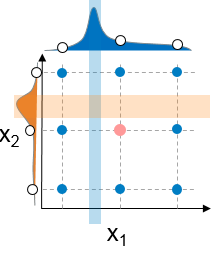
\includegraphics[width=\linewidth]{graphics/Background/hyperparameter-grid-search.png}
		\caption{Grid.}
		\label{bg: fig:automated parameter tuning approaches: grid}
	\end{subfigure}
	\begin{subfigure}[b]{0.25\linewidth}
		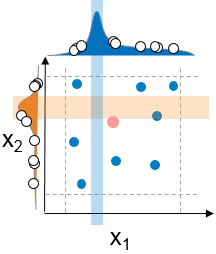
\includegraphics[width=\linewidth]{graphics/Background/hyperparameter-random-search.png}
		\caption{Random.}
		\label{bg: fig:automated parameter tuning approaches: random}
	\end{subfigure}
	\begin{subfigure}[b]{0.25\linewidth}
		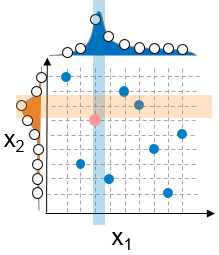
\includegraphics[width=\linewidth]{graphics/Background/hyperparameter-learning-search.png}
		\caption{Learning.}
		\label{bg: fig:automated parameter tuning approaches: learning}
	\end{subfigure}
	\caption{Automated Parameter Tuning Approaches.}
	\label{bg: fig:automated parameter tuning approaches}
\end{figure}

\paragraph{Grid search parameter tuning.} It is a rather simple approach for searching parameters. Here, the original search problem is relaxed and later solved by a brute-force algorithm. The set of all possible configurations (parameter sets) for relaxed problem is derived by specifying a finite number of possible values for each hyper-parameter under consideration. After evaluating all configurations on TS, the best-found solution is reported. Hence, this approach could skip promising parts of search space (\cref{bg: fig:automated parameter tuning approaches: grid}). Moreover, the required time to probe all possible combinations is increasing by means of a factorial complexity.

\paragraph{Random search parameter tuning.} This methodology relies on a random (often uniform) sampling of hyper-parameters and their evaluation on each iteration. At first sight, it might seem unreliable to chaotically traverse the search space. But empirical studies show that with a growing number of evaluations this technique starts to outperform grid search~\cite{bergstra2012random}. As an example, let us draw your attention to the best configurations (highlighted in pink) found by grid (\cref{bg: fig:automated parameter tuning approaches: grid}) and random search (\cref{bg: fig:automated parameter tuning approaches: random}) techniques. The best randomly sampled configuration is definitely better than the one found by the grid search.

\paragraph{Heuristic search parameter tuning.} By their nature, heuristic algorithms may be applied to tackle the most black-box search problems. Since the parameter tuning is one concrete type of search problem, it is also often tackled by a high-order heuristic approaches (meta-, hybrid-, hyper-heuristics) \cite{crawford2013parameter1,crawford2013parameter2,carrizosa2014nested}. The advantage of heuristics usage lays in their ability to learn during the optimization process and use an obtained memory to guide the search more efficiently.

\paragraph{Model-Based Search Parameter Tuning.} In most cases, the dependencies between tuned parameter values and optimization objective do exist and can be utilized for hyper-parameter tuning. By predicting which parameter combinations lead to better results, model-based tuning could make precise guesses. As it is shown in \cref{bg: fig:automated parameter tuning approaches: learning}, after accumulating enough information the learning algorithm starts making more precise guesses, which in contrast to previously outlined model-free approaches are desirable and more robust.

\paragraph{} Naturally, this optimization problem could be tackled by almost every approach discussed in this thesis. However, taking into account the fact that (1) TS is often a \textit{black-box} we eliminate exact and approximate solvers, (2) the evaluation cost is high, therefore, it is not desirable to apply the aforementioned heuristics directly, since they require performing a high number of TS evaluations to find a good configuration. With this idea in mind, researchers started to (1) create optimization algorithms that traverse the search space of configurations more efficiently and (2) build models that could imitate the dependencies between parameters and objective values, a so-called \textit{surrogate models}. The former direction is nothing else but an enhancement to already existing optimization techniques, which allows accumulating and utilization of more information, obtained during an optimization. The latter approach is crucial for problems where TS is expensive to evaluate.
It is often used as an enhancement in optimization algorithm, enabling one to simulate evaluation of real system instead of expensive direct evaluations. Still, it is a frequently used approach to combine the previously reviewed search space traversal techniques, such as evolutionary algorithms, simulated annealing, tabu search with the surrogate models for optimization.


\subsection{Systems for Model-Based Parameter Tuning}\label{bg: parameter tuning expamples}
Parameter tuning is an obligatory task when the maximum system performance is a must-have requirement and should be performed at the design time.
Novel tuning approaches are usually developed in form of frameworks with exposed hooks for attaching the TS.

Since the target system evaluations here supposed to be costly, parameter tuning frameworks are trying to utilize every single bit of information from evaluations and a creation of surrogate models and using efficient optimization approaches is obligatory.

In this section we review some existing open-source parameter tuning systems from the following perspectives:
\begin{itemize}
	\item \textbf{Conditional parameters support} is provided to user and handled by tuning system ability to describe conditional dependencies between hyper-parameters. As an example, imagine \emph{crossover type} parameter of genetic algorithm that takes only some specific values: partially mapped crossover (PMX), Cycle Crossover (CX), etc. Binding a certain crossover type, one will require providing parameters for this specific crossover type, as well as to eliminate the respective parameters for other crossover types. This type of dependency could be described in form of a parent-child relationship, however, other types of dependencies also exist.
	
	\item \textbf{Parameter types support} is one of the basic tuning systems usability requirements. In detail, TS parameters could be not only a numerical (integer or fractional) but also a categorical in form of strings, boolean values, etc. Considering categorical data types, they could be either \emph{nominal}, which depict only possible atomic values, or \emph{ordinal}, which imply also value comparison but no distance notion. For instance, let us refer to genetic algorithm parameters. \emph{Population size} is of numerical integer type in a range $[1..\infty)$, \emph{mutation probability} is of numerical fractional type in a range $[0..1]$, \emph{crossover type} is of categorical nominal type with \texttt{\{PMX,CX\}} choices. Please note, we could also view the population size as a set of finite values \texttt{\{10,100,1000\}} therefore, turning it into the categorical ordinal parameter.
	
	\item \textbf{Extensibility} is crucial when one would like to try a new promising and intriguing learning algorithm for guiding a search that was not available in the parameter tuning system yet. Practically, one may need not only new learning algorithm, but some other features like a non-trivial stopping criterion, tools for handling stochastic behaviors, or different strategies for random sampling (which are used to replace a model-based prediction, while the tuning system is learning).
	
	\item \textbf{Parallel evaluations} required for utilizing available computational resources that could scale horizontally, providing simultaneous evaluation of multiple configurations. This often could speeds-up the learning process.
\end{itemize}

Among reviewed systems, we could distinguish those, which were created directly to face the parameter tuning problem and the others that are more generic optimizers but still applicable in parameter tuning cases.
A specific optimizer will be used for searching the parameters, if it exposes several features. Firstly, it must consider an optimization function evaluation to be expensive and tackle this problem explicitly. For instance, using surrogate models or the other TS approximations. Secondly, a potential tuner should be able to tackle dependencies and conditions among parameters.

\subsubsection{SMAC}\label{bg: smac}
Sequential Model-based Algorithm Configuration (SMAC\footnote{SMACv3 GitHub repository~\url{https://github.com/automl/SMAC3/}})~\cite{hutter2011sequential} is a system for parameters tuning, developed by the AutoML research group (here we review the $3^{rd}$ version of SMAC). 

In their research, scientists generalized the process of parameter tuning under the  \emph{Sequential Model-Based Optimization} (SMBO) term as the iterations between (1) fitting models and (2) using them to choose the next configurations for evaluation. 
This term naturally formalizes most of the existing (except MBMO, but we do not tackle multi-objectiveness in this thesis) parameter tuning approaches and may be used as a distinguishing characteristic of optimization algorithms, since they naturally could be applied not only to the parameter tuning problems.

SMACv3 is an extension introducing the learning models and sampling mechanisms to previously existing random online aggressive racing (ROAR) algorithm. The authors showed that a machine learning in general and regression models in particular (playing the role of surrogates) are applicable not only to parameter tuning but also to optimize any expensive black-box function. 

The development of this system was motivated by the limitations of all existing SMBO approaches. Among them an expanding the applicability to categorical, but not only to numerical parameters. Also, to reduce a variance influence the target algorithm performance optimization may be performed on a number of problem instances (benchmark set), instead of a single instance.

A routine in SMAC could be viewed as an iterated application of three steps: (1) building a learning model, (2) using it for making choices regarding which configurations to investigate next and (3) actual evaluation of TS.

The evaluation (3) here is carried out by the original ROAR mechanism, where the running of each new candidate solution continues until enough data (from benchmark set of problem instances) is obtained to either replace the current solution or reject the candidate. On contrary to model-less ROAR, SMAC at step (1) builds the regression random forest surrogate — an instance of a machine learning algorithm~\cite{breiman2001random}. The usage of the regression decision trees is motivated by the fact that they fit well to categorical data and complex dependencies in general. Later, at step (2) an iterative local search (ILS) heuristic is applied in combination with \emph{expected improvement} (EI) evaluation (part of the Bayesian optimization process)~\cite{shahriari2015taking}. The EI is a measurement of possible solution quality improvement obtained by an underlying configuration, therefore, higher EI means that the candidate is better. ILS starts at the best previously found configuration and traverses its neighborhood distinguishing between configurations using EI and regression model built at step (1). SMAC compares configurations by means of the objective value and considers only minimization case. EI is large for those configurations, which have a low predicted cost and for those, with high uncertainty in results, therefore, providing the exploration-exploitation balance~\cite{jones1998efficient}.


\subsubsection{IRACE}\label{bg: irace}
IRACE\footnote{IRACE GitHub repository~\url{https://github.com/MLopez-Ibanez/irace}} is a hyper-parameter tuning package~\cite{lopez2016irace} as the implementation of the iterated racing algorithm~\cite{birattari2010f}.

The underlying methodology is somewhat similar to the one implemented in SMACv3 and comprise three main steps: (1) sampling new configurations using prior knowledge, (2) empirically finding the best ones among the sampled using the racing algorithm and (3) updating the prior knowledge to bias future samples towards better configurations. The prior knowledge here is represented as a probability distribution of values for each parameter independently (truncated normal and discrete distributions for numeric and categorical parameter types respectively). During step (3), the probability distributions are build using the best found in step (2) configurations, increasing the sampling chance for promising values.

Iterated racing step (2) here is a process of running the target system using sampled configuration on a set of problem instances. After solving each instance, the statistically worse-performing configurations are rejected and racing proceeds with remaining ones. This process continues until it reaches the predefined number of survivors, or after solving a required amount of problem instances (in this case all remaining configurations are considered to be good). 

IRACE supports various data types, such as numerical or categorical and the possibility of conditions description as well. While the problem of data types is resolved by the usage of different underlying distribution types, the conditional relationships are handled by the dependency graphs. During step (1), non-conditional parameters are sampled firstly and only afterwards, if the respective conditions are satisfied, the dependent parameters are sampled.


\subsubsection{HpBandSter}\label{bg: bohb}
A distributed Hyperband implementation on Steroids (HpBandSter\footnote{HpBandSter GitHub repository: \url{https://github.com/automl/HpBandSter}}) is a realization of BOHB algorithm~\cite{falkner2018bohb} in the software framework.
While SMAC outperforms and partially reuses the decisions made in ParamILS~\cite{hutter2009paramils}, BOHB (Bayesian optimization combined with Hyperband) is the parameter tuning tool that outperforms SMAC and was created by the same AutoML research group.

As it stated in the framework name, the SMBO routines are carried out with mainly two algorithms: learning and configurations sampling is performed by the Bayesian optimization (BO) technique \emph{tree parzen estimator} (TPE), while evaluation of sampled configurations and their comparison is carried out by the Hyperband (HB) algorithm.

The TPE usage instead of naive Gaussian processes-based BO and expected improvement evaluation was motivated by a better dimensional scaling abilities and an internal support of both numerical and categorical parameter types. However, some minor transformations are still required.
Unlike vanilla BO, where the optimization is done by modeling the result distributions given the configuration parameters, TPE builds two distributions of parameter values. It splits the configurations into two sets distinguishing their `goodness'. During the sampling, it proposes those parameter values, which have a high probability to be in the `good' distribution and simultaneously low probability to be in the `bad' one. For more detailed explanation, we refer to TPE description given in~\cite{bergstra2011algorithms}.

A central part of BOHB, namely the Hyperband algorithm, is a promising bandit-based strategy for hyper-parameter optimization~\cite{li2017hyperband}, in which the \emph{budget} for entire parameter tuning session is defined beforehand and divided between iterations. The role of the budget could play any setting that controls the accuracy of a configuration evaluation by TS, where estimation with the maximal budget provides the most precise evaluation, while the minimal budget gives the least accurate approximation of configuration results.
The running examples of budget could be a number of iterations in iterative algorithm, a number of epochs to train the neuron network, or a number of problem instances from benchmark set to evaluate. As a result, the requirements in TS arise to expose and support budget usage as expected in BOHB.

At each iteration, in original version HB samples a number of configurations uniformly at random. The authors introduced an \emph{intensification} mechanism according to which, a number of per-iteration sampled configurations decreases for the later iterations, while the amount of budget given for iteration remains the same. As an outcome, first iterations of HB are full of coarse-grain evaluated configurations, while the later iterations produce a higher number of more precise measurements. Each iteration of HB is split to the number of \emph{successful halving} (SH) procedure executions, which at each execution drop poorly performing configurations (usually $\sfrac{2}{3}$). As one may expect, since the number of measured configurations in subsequent iterations decreases, the amount of SHs execution drops too, therefore, the remaining configurations are evaluated more precisely.

The binding of Hyperband and Bayesian TPE is made in several places. Firstly, the learning models are updated each time, when new results are available for every budget value. Secondly, at each HB iteration instead of random sampling, the TPE model is used to pick next configurations. Please note that BOHB uses only the surrogate, which was built on the configurations evaluated with the largest budget. This decision results in more precise surrogate models and, therefore, better predictions in the later stages of parameter tuning process.


\subsubsection{BRISEv2}\label{bg: brise}
The great part of software potential lays not only in its ability to tackle a problem at hand, but also on the general usability and adaptivity to unforeseen tasks.
Here we review the $2^{nd}$ version of BRISE\footnote{BRISEv2 GitHub repository: \url{https://github.com/dpukhkaiev/BRISE2/releases/tag/v2.3.0}}~\cite{brise2spl}, since the very early BRISE versions (major version 1~\cite{brise1monolite}) were more monolithic and hard to apply for parameter tuning problem at hand.

While designing this system, authors were focused not solely on learning mechanisms for parameter prediction, but on the overall system modularity as well.
Being a software product line (SPL), BRISE was designed as a set of interacting components (nodes), each acting according to its own specific role. 
The system could be viewed from two perspectives. One is a birds-eye view on all available nodes with their roles and the other is a fine-grained description of~\textit{main-node} concretely.

Before reviewing each perspective, it is worth justifying the central terms used in the system. Please note that some of them are similar to the one defined above, but they were explicitly implemented in form of interacting entities.
\begin{itemize}
	\item \textbf{Experiment} encapsulates the information about a certain run of BRISE. For instance, within a parameter tuning session it carries such information as BRISE experiment description (a specification of parameter tuning procedure in JSON format), evaluated during session configurations with their results.

	\item \textbf{Configuration} is a combination of input parameter values for TS. It could be run several times to obtain a statistical data, therefore, contains number of \emph{Tasks}. Naturally, the configurations are comparable in terms of the results averaged over performed runs.

	\item \textbf{Task} is a single evaluation of TS under provided configuration for specified in description problem scenario.

	\item \textbf{Parameter} is a meta-description of certain configuration part and a building block for search space. It defines a set or range of possible values.

	\item \textbf{Search space} comprises all parameters and their dependencies and could verify the validity of configuration.
\end{itemize}

From a birds-eye view perspective, BRISE consists of \emph{main-node} as the system backbone, several \emph{worker-nodes} as target algorithm runners under provided configurations, \emph{event-service} to distribute tasks between available worker-nodes, \emph{front-end-node} to control and report optimization process on a web-page, and non-obligatory \emph{benchmark-node} that could be handy for executing and analyzing a number of experiments.

The main-node is a combination of objects, which interact in terms of queue callbacks. Therefore, when a new configuration is evaluated, the new model is built and used for the next configuration prediction. The intent of introducing the aforementioned terms is to use them as a core of the framework, while such components as \emph{prediction models}, \emph{termination criteria}, \emph{repetition management} or \emph{outliers detection} are exposed to client for the variability reasons. Naturally, the developers also created a set of available out-of-the-box implementations for each variability component.

To use BRISE for parameter tuning, one should (1) construct an experiment and search space descriptions in JSON format and (2) add the respective target system evaluation logic in \emph{workers}. All the rest will be carried out by the system.
% TODO: we deffinitely should formalize Tasks, since this entry is exposed to user (it should parse it to retrieve prameters as well as add results).


\subsection{Parameter Control}\label{bg: parameter control}
Generally speaking, the biggest disadvantage of parameter tuning approaches is defined by the fact that they usually require many TS runs to evaluate its performance with different configurations. On the other hand, the parameter control approaches are able to solve this issue but the drawback lays in their universality.

The advantageous characteristic of any system is its ability to adapt at runtime.
It could happen so that an algorithm with tuned parameters performs well at the very beginning of a problem-solving process, but struggles in the later stages. The other algorithm configuration may result in an opposite behavior. This could be caused by various reasons and it is often hard to tell, which of them the algorithm is facing at the moment. 

In contrast to the parameter tuning approaches, where optimal parameters are \emph{firstly} searched and only afterwards are used to solve the OP, the parameter control is an approach of searching the parameters \emph{while} solving the OP. It also could be expressed as a system reaction to the changes in a solving process. Sometimes, it is named an \emph{online} parameter tuning. The drawback of this approach lays in a lack of generality, since often a parameter control technique is embedded into an algorithm, therefore, is algorithm-dependent.

The only broad classification facet we were able to distinguish is the \emph{type of control mechanism}, where the \emph{deterministic} and \emph{adaptive} strategies exist. The first type suggests changing the parameters in a predefined schedule, while the second type assigns the parameter values upon received feedback. To the best of our knowledge, the adaptive approaches are mostly dependent on the concrete algorithm instance. Therefore, it is hard to present a generic classification of parameter control approaches for all algorithms. However, this could be done for each particular algorithm family.

We provide an insight into the parameter control reviewing the examples of proposed strategies for some meta-heuristics. For the more comprehensive review of the recently published strategies we encourage the reader to examine the source paper, used here~\cite{huang2019survey}.


\subsubsection{Parameter Control in Simulated Annealing}\label{bg: parameter control: SA}
The most frequently controlled parameters in simulated annealing algorithms are the \emph{cooling rate} (the velocity of temperature decrease) and the \emph{acceptance criteria} (decision, whether to accept a proposed solution, or not).

The control in cooling rate parameter is motivated as follows: if the temperature decreases too rapidly, the optimization process may settle in the local optima, but too low cooling rate is a computationally expensive, since SA requires more TS evaluations to converge. Among deterministic approaches, researchers mainly distinguish linear, exponential, proportional, logarithmic and geometrical cooling schedules. In contrast to deterministic approaches, in~\cite{karabin2020simulated} the authors proposed an adaptive strategy to change the cooling rate, based on the statistical information, evaluated on each optimization step. Specifically, if the statistical analysis named in research a \emph{heat capacity} shows that the system is unlikely to be trapped in the local optima, the cooling rate is increased. On the contrary, it is decreased if the possibility of being trapped is high.

In~\cite{ghandeshtani2019entropy} the authors propose an adaptation of another hyper-parameter: acceptance criteria. The utilized mechanism is based on thermodynamics fundamentals, such as \emph{entropy} and \emph{kinetic energy}. The authors suggest replacing the standard acceptance criteria (based on the current temperature and the solution quality) with the one based on the solutions entropy change evaluation.

Many researches were made to investigate, which is the best among deterministic and adaptive strategies~\cite{thompson1995general,ingber2000adaptive,de2003placement,azizi2004adaptive,lou2016parallel}. In many cases, the authors conclude that the adaptive methods provide more robust and promising results.


\subsubsection{Parameter Control in Evolutionary Algorithms}
While searching the parameter control examples in heuristics, one will find dozens of proposed methodologies for the evolutionary algorithms. It is arising from the fact that an idea of changing the algorithm parameters dynamically came from EAs~\cite{karafotias2014parameter}. The motivation for such a number of performed studies lays in a strong dependence of an algorithms' performance on parameter values. 

The deterministic and adaptive mechanisms in EAs are extended by the $3^{rd}$ type — a \emph{self-adaptive} approach. It implies an encoding of parameter values in the solution genomes, allowing them to co-evolve with the solutions at runtime~\cite{doerr2020theory}. All the proposed strategies could be split into two families: one includes the algorithms proposing to adapt a concrete parameter solely and the other, which includes the approaches to control a group of parameters. In EAs the commonly implicated hyper-parameters are \emph{population size}, \emph{selection strategies} and \emph{variation aspects} (namely crossover and mutation operators). In case of interest, we propose the reader to analyze recently conducted reviews and researches dedicated to parameter control in evolutionary algorithms~\cite{karafotias2014parameter,aleti2016systematic,smith2020self,doerr2020theory}.

There is one rather intriguing parameter control approach proposed for the evolutionary algorithms. In~\cite{karafotias2014generic} the authors introduce a reinforcement learning (RL) parameter controller, whose goal is to select the EA parameters online evaluating a set of simple observables. They include: a genotype diversity, a phenotype diversity, a fitness standard deviation, a fitness improvement and a stagnation counter.
The RL in this work adheres the following \textbf{MAPE-K} methodology~\cite{brun2009engineering}. On each iteration the observables are \textbf{M}onitored, their values are \textbf{A}nalyzed to build a parameter control \textbf{P}lan, which is \textbf{E}xecuted in the next iteration. The letter \textbf{K} denotes a central part of this methodology — the knowledge.
This set of proposed observables could be split into two logical groups. One is the algorithm-specific with the genotype/phenotype diversities and the fitness standard deviation, while the other is algorithm-independent and includes the fitness improvement and the stagnation counter. We believe the proposed RL approach could be applied to other algorithms, with the only requirement in exposing the observable knowledge. The proposed in~\cite{karafotias2014generic} parameter control methodology may be one of the first to generalize a parameter control techniques and later in~\cref{concept:parameter control} we use it as a part of our approach.


\subsection{Conclusion on Parameter Setting}\label{bg: parameter setting conclution}
At this point, we finalize our review of the parameter settings problems with three conclusions:
\begin{enumerate}
	\item The parameter tuning area is investigated widely and nowadays the research settles in the form of combining different learning models to implement the SMBO algorithms in framework-like tuning systems.
	
	\item The parameter control is actively driven by two motivations. Firstly, the runtime changes in solving process are unpredictable; therefore, the control is believed to better fit them, comparing to the statically defined by parameter tuning techniques. Secondly, the resources spent for offline parameter settings are high, but they are paid-off by a high quality of algorithm configuration. Therefore, from this perspective, the control approaches are trying to reach the quality of the offline settings, spending fewer resources. Unfortunately, nowadays the online approach is not generic to be commonly applicable.
	
	\item The decision on concrete technique is use-case specific and is driven by the amount of available resources and the required setting quality as well.
\end{enumerate}

\section{Combined Algorithm Selection and Hyper-Parameter Tuning Problem}\label{bg: section cash}
The goals of automatic machine learning are quite similar to persecuted by hyper-heuristics. They both operate on search space of algorithms (or their building blocks), which later are combined, with an objective to find the best performing ones, and used to solve the problem at hand. 

In this section we review one particular representative of automatic machine learning systems.
Based on the ML framework Scikit-learn~\cite{scikit-learn}, Auto-sklearn system~\cite{feurer2015efficient} operates over a number of classifiers, data and features preprocessing methods \textbf{including their hyper-parameters} to construct, for provided dataset, the best performing (in terms of classification accuracy) machine learning pipeline.
This problem was formalized as \textit{combined algorithm selection and hyper-parameter tuning problem} (CASH) and presented previously in Auto-WEKA~\cite{thornton2013auto} system. Intuitively, it could be rephrased as follows: ``For a given optimization problem, find the best performing algorithm and its hyper-parameters among available and solve the problem''. 

Please note, to the certain extent Auto-sklearn is similar to HHs, which use LLHs for traversing the search space and solving the OP. However, the automatic machine learning techniques operate on the completion algorithms, the results of which are evaluated at the end of their run. On the contrary, online HHs are able to evaluate the intermediate performance of low-level heuristics, since they are anytime algorithms.
CASH problem seems to be a combination of problems solved by HHs and parameter tuning approaches. We also found that the architecture search problems~\cite{elsken2018neural} (related to neural networks) are nothing else but particular case of CASH.


Turning back to Auto-sklearn, the crucial decisions made here is the combination of offline and online learning, resulted an exceptional performance of Auto-sklearn in classification tasks.

During the offline phase, for each of available datasets published by the OpenML community~\cite{OpenMLPython2019}, search of the best performing machine-learning pipeline was done using the BO technique implemented in the discussed previously SMAC framework~\cite{hutter2011sequential}.
After that, the \textit{meta-learning} was executed to derive the meta-features for each dataset.

The resulting combination of the datasets, machine learning pipeline and meta-features were stored and later used to initialize the online phase of pipeline search.
The information from the meta-learning phase is used as follows: for a given new dataset, the system derives the meta-features and selects some portion of created during the offline phase pipelines that are the nearest in terms of meta-feature space. Then, these pipelines are evaluated on a new dataset to initialize the BO in SMAC. This decision results in the ability to evaluate well-performing configurations at the beginning of the tuning process.

During the online phase, another crucial improvement was introduced. 
Usually, while searching the best-performing pipeline, a lot of effort is spent in order to build, train and evaluate intermediate pipelines. After each evaluation, only the results and the pipeline description are stored, but the pipeline itself is discarded. In Auto-sklearn, however, the idea lays in preserving previously instantiated and trained pipelines, obtained while solving the CASH problem. Later, they are used to form an ensemble of models and tackle the problem at hand together. This means that the results of this architecture search are a set of models with different hyper-parameters and preprocessing techniques, rather than a single model. This ensemble starts from the worst performing ones (obtained at the beginning of the search) and ends with the best suited model for the respective dataset. Naturally, each ensemble members' influence on the final results is weighted.

The potential of offline phase is derived entirely from the existence of such a dataset repository and depends on the availability of homogeneous datasets. The proposed online methodology, which mimics the regression trees, is more universal and could be reused widely.

In general, an empirical investigation of Auto-sklearns' universality would be rather intriguing, since the only cases of Auto-sklearn application we managed to find are the classification tasks but not regression problems~\cite{feurer2015efficient,biedenkapp-ecai20}.

The field of automated machine learning is one of trending research directions, that is why there exist dozens of open-source systems, such as \textit{Auto-Weka}~\cite{thornton2013auto}, \textit{Hyperopt-Sklearn}~\cite{komer2014hyperopt}, \textit{Auto-Sklearn}~\cite{feurer2015efficient}, \textit{TPOT}~\cite{olson2019tpot}, \textit{Auto-Keras}~\cite{jin2019auto}, etc. Among open-source, there are many commercial systems, such as \textit{RapidMiner}, \textit{DataRobot}, Microsoft’s \textit{Azure Machine Learning}, Google’s \textit{Cloud AutoML}, and Amazons' \textit{Machine Learning on AWS}.


\section{Conclusion on Background and Related Work Analysis}\label{bg: conclusion}
In this chapter we have presented the review of optimization problems, their concrete instances and existing solver types focusing on the heuristics.
There exist several levels of generality in heuristic solvers: simple heuristics, meta-heuristics and hyper-heuristics.

The applicability of each algorithm is problem-dependent and derives from the exploration-exploitation balance and strength, revealed in a particular case.
It is difficult to guess beforehand, which heuristic will outperform the others in an unforeseen use-case.
With respect to this, hyper-heuristics seems to be the most perspective and universal solvers, since they do not tackle the problem directly, but rather select and apply the best suited among controlled algorithms.

From the other perspective, the solver performance is also dependent on the values of its parameters.
It turns out, that the parameter setting is also an optimization problem.
There exist several ways to solve it: (1) set the values manually, based on experience and intuition, (2) utilize the parameter tuning systems, which find the best values automatically and later use those found parameters, or (3) exploit the parameter control mechanisms.
Among all strategies, the last seems to be the happy medium, since tuning requires lots of expensive algorithm executions to produce good parameter settings, while manually choosing hyper-parameters is an error-prone process that requires experienced guidance. The analysis of parameter control approaches showed that the existing techniques are heuristic-dependent, therefore, our first research question is defined as follows \textbf{RQ1} \emph{Is it possible to perform the algorithm configuration at runtime on a generic level?}

The outcome of no-free-lunch theorem cannot be ignored, according to which no single algorithm can tolerate a broad range of problems equally outperforming other solvers. That is why we cannot set aside hyper-heuristics, which are designed to find the best solving algorithm suited for a particular optimization problem case.

The research in automatic machine learning has made a step further and tends to combine both algorithm selection and parameter tuning problems into a single CASH problem, formalized in~\cite{thornton2013auto}. The search space in CASH problem is formed of algorithm variants and their respective hyper-parameters. However, one solver cannot use the parameters of another, thus, the resulting search space happens to be `sparse'. In general, the structure of CASH problem is almost the same as regular parameter tuning case. That is why the commonly used solvers for CASH problems are the parameter tuning systems: SMAC in Auto-sklearn and Auto-Weka, Hyperopt in Hyperopt-Sklearn and so forth.
Not many surrogate models are able to handle the sparse search spaces: random forest machine learning model and Bayesian optimization approaches with exotic kernel density estimators~\cite{levesque2017bayesian}. Even fewer optimizers are able to perform well in such sparse spaces.
%However, none of reviewed parameter tuning systems uses optimizer that is able to perform an efficient search in such `sparse' spaces.
The other drawback is that the CASH problem definition is limited to searching the algorithm and its parameters in an offline manner.

We believe that the solutions of both algorithm selection and parameter setting problems is highly dependent on a problem at hand.
That is why a search for the best tool (solver) and its setting (parameters) should be performed in an online manner, in other words, while solving the optimization problem. Since the generic parameter control concept was not proposed yet, naturally, we were not able to find the techniques to merge and solve both the algorithm selection and parameter control problems in runtime. Therefore, we defined our second research question \textbf{RQ2} \emph{Is it possible to simultaneously perform algorithm selection and parameters adaptation while solving an optimization problem?}

As CASH merges algorithm selection and parameter tuning techniques to get the outstanding performance, we found a merge of online algorithm selection and parameter control an intriguing and worth-to-try idea. However, the amount of spent resources and the imprecision of surrogates estimations for simultaneous search of both the algorithm type and its parameter values may be discouraging. To explicitly evaluate this, we define the final research question as \textbf{RQ3} \emph{What is the effect of selecting and adapting algorithms while solving an optimization problem?}

\paragraph{}
\textbf{Research objective defined.}

In this thesis we are trying to achieve the best of both online algorithm selection and parameter control worlds. The resulting approach should be able to solve an optimization problem, applying \emph{the best suited low-level-heuristic} and \emph{setting its parameters} at \emph{runtime}. With this idea in mind, we investigate a possibility of turning existing parameter tuning system into an \textbf{online selection hyper-heuristic with parameter control in low level heuristics}.

  \chapter{Concept Description}\label{Concept description}
While there exist no universal approach to control the algorithms parameters (\cref{bg: parameter setting conclution}), our conclusion on the literature analysis was the absence of existing approaches to combine both on-line techniques for the algorithm selection and the parameter settings (\cref{bg: conclusion}). 

In this Chapter we propose the methodology to resolve this problem, excluding the implementation details.

In \cref{concept:parameter control}, we introduce the generic parameter control technique and expand it with the use-case of algorithm selection. As concluded in \cref{bg: conclusion}, the main weakness of the reviewed approaches to tackle CASH problems lays in the inability of learning mechanisms to fit and predict in sparse search spaces. The same issue arises in case of on-line algorithm selection and parameter settings, and we resolve it on two levels: firstly in the search space structure and secondly in the prediction process. In \cref{concept:search space} we present the joint search space of both algorithm selection and parameter control problems. We outline the functional requirements for such space. Next, we describe the related prediction process in \cref{concept:prediction}. While decoupling the learning models from the search space structure, we provide the certain level of flexibility in the usage of different learning models.
% TODO: check if needed in this chapter
Finally, in \cref{concept: llh} we direct our attention to the low level heuristics (LLH) — a working horses of the desired hyper-heuristic. We highlight the requirements to LLH that are crucial in our case.


\section{Combined Parameter Control and Algorithm Selection Problem}\label{concept:parameter control}
The base idea of the parameter control approaches lays in the solver behavior adaptation as the response to changes in the solving process (\cref{bg: parameter control}). As we mentioned during the heuristics review (\cref{bg: section heuristics}), the algorithm performance is highly dependent on the provided exploration-exploitation balance, which in turn, depends on (1) the algorithm itself and (2) its configuration. The task of parameter control is to find the later, which provide the best performance.

In our work, we solve the parameter control problem utilizing a similar to proposed in~\cite{karafotias2014generic} reinforcement learning (RL) approach for evolutionary algorithms.
The underlying idea of RL could be described as a process of performing actions in some environment in order to maximize the reward, obtained after each performed action. To apply this technique onto the parameter control problem, we must define what are those \emph{actions} and how to estimate the \emph{reward}. Thus, for making the parameter control applicable to broad range of algorithms, we analyze not the solver state itself but the optimization process (in~\cite{karafotias2014generic}, the authors use both algorithm-dependent and generic metrics). To realize the MAPE-K control loop, we must interrupt the solver, analyze the intermediate results, learn the current trend among parameters, configure the solver with the most promising parameter values and continue solving. The number of MAPE-K loop iterations $i$ define the granularity of learning, where one should balance between \emph{time to control} (TTC) the parameters vs \emph{time to solve} (TTS) the problem. Naturally, the limitation of proposed approach is the use-cases, where $TTS >> TTC$.

\todoy{Should I highlight the limitation(s) here or in conclusion and refer from here?}

To evaluate the gained in iteration $i$ reward, instead of using straight solution quality value, we calculate the quality improvement, obtained with the provided configuration $C_i$. When the search process converges towards the global optimum, the improvement value tends to decrease, since the amount of significantly better solutions drops. Using the improvement values directly or could confuse the learning models and therefore, cause the prediction quality to struggle. To resolve this issue, the relative improvement (RI) of solution quality is calculated using \cref{concept: RI formula}, where $S_{i-1}$ and $S_i$ are the solution qualities before and after $i^{th})$ iteration respectively.

The evaluated $C_i \rightarrow RI$ pairs in previous iterations are then used to predict the configuration for next iteration $C_{i+1}$. At this point, we made two decisions in the sampling process: (1) hide the search space shape and (2) use the surrogate models for finding configurations that lead to the highest reward.

\begin{equation}
RI = \frac{S_{i-1} - S_{i}}{S_{i-1}}
\label{concept: RI formula}
\end{equation}

After sampling the $C_{i+1}$ configuration, we set it as the solver parameters. To proceed with the solving process, we seed the solver with the solutions from $i-1$ iteration as well.

When it comes to the algorithm selection problem (discussed in \cref{bg: hh}), we treat the solver type itself as the subject of parameter control and use the proposed RL approach to estimate the best performing algorithm. However, when we add the solver type as a parameter, the resulting search space become sparse and requires special treatment. Two commonly used approaches for tacking this problem exist. The first requires special type of learning models, while the second suggests the problem transformation in a way of excluding the undesired characteristics.

During the review of model-based parameter tuning approaches (\cref{bg: parameter tuning}), we made a conclusion that all reviewed systems follow strictly the first idea. For instance, as the surrogate models, BOHB~\cite{falkner2018bohb} and BRISE~\cite{brise2spl} use the Bayesian probability density models. Those surrogates could naturally fit to the described search space shape, but the proposed approaches are not able to make the predictions effectively, since the most of predicted configurations will violate the dependencies. As the illustration, imagine after $i^{th}$ iteration, the surrogate models learn about two superior parameters: one indicates a well-performing heuristic type (the Genetic Algorithm), the other — an effective configuration for another algorithm type (an exponential cooling rate for the Simulated Annealing). In this case, the reviewed systems sampling methods will tend to predict the invalid configurations with those two parameter values.

In this thesis we follow the second approach namely, the problem transformation in order to sample the valid configurations only. The following Section depicts a required preparation step, made in the search space, while the later is dedicated to the prediction process.


\section{Search Space Structure}\label{concept:search space}
When the time comes to selecting not only the solver parameters but also the solver itself, the united search space no longer could be presented as `flat' set of parameters since it tends to appearance vast amount of invalid parameter combinations. Let us estimate the number of all possible configurations vs the amount of meaningful ones. Suppose, we have the $N_s$ number solver types, each exposing the $N_{s,p}$ number of hyper-parameters with the $N_{s,p,v}$ number possible values. The aggregated quantity of configurations $N_c$ in the disjoint search spaces is calculated as the number of possible combinations using \cref{c: disjoint search space size}.

\begin{equation}
N_c = N_s \cdot \prod_{1}^{N_{s,p}} N_{s,p,v}
\label{c: disjoint search space size}
\end{equation}

However, if we decide to tune (or rather to control) the solver type itself, the resulting quantity of possible configurations is calculated using \cref{c: joint search space size}.

\begin{equation}
N_c = \prod_{1}^{N_{s}} \prod_{1}^{N_{s,p}} N_{s,p,v}
\label{c: joint search space size}
\end{equation}

For the better intuition, lets try some numbers. By setting all $N_s = N_{s,p} = N_{s,p,v} = 3$ (the rather small example), the amount of configurations estimated separately for each solver equals to $N_c = 81$ (\cref{c: disjoint search space size}). However, if we join the solver parameter spaces, \cref{c: joint search space size} shows the significant growth in the search space size: $N_c = 19683$. Note, the number of \emph{really unique} configurations remains the same thus, in the joint space it is only $\approx 0.4\%$. By setting the $N_s = N_{s,p} = N_{s,p,v} = 4$, this number drops to $\approx 9 \cdot 10^{-8}\%$. It could decrease even further if the dependencies among hyper-parameters exist. In such case, the predictive abilities of models may straggle.

To overcome this, we utilize similar to the utilized in IRACE~\cite{lopez2016irace} framework idea: \emph{explicitly indicate the dependencies as a parent-child relationship among the search space entities $p$, firstly predict the parent parameter, afterwards — the children.} This give us an opportunity to threat the algorithm type as the regular categorical parameter, makes the search space structure uniform and simplifies the prediction process.

This decision sets the following search space \emph{structural requirements}:
\begin{enumerate}
	\item[S.R.1] The \textbf{parent-child relationship} must describe the dependencies between different parameter types.

	\item[S.R.2] The \textbf{uniform parameter types} simplifies the structure and hides the domain-specific intent of each parameter thus, algorithm type and its hyper-parameters are treated in the same way.

	\item[S.R.3] The \textbf{value-specific dependencies} describe a concrete parent value(s), when the child should be exposed. For instance, the parameter \textit{algorithm type} has a number of possible values, each of them requires own set of hyper-parameters, which should remain hidden for the other solver types.
\end{enumerate}

\svgpath{{graphics/Concept/}}
\begin{figure}
	\centering
	\includesvg[width=1.0\textwidth]{feature tree}
	\caption{Search space representation.}
	\label{concept:pict:Search Space Representation}
\end{figure}

\cref{concept:pict:Search Space Representation} shows an example of such search space with $s$ algorithm types, each having $p$ parameters with $v$ possible values. The entities with triangles $\bigtriangledown$, namely the concrete values of parameters, form the joint-points to which the other parameters could be linked. 


\section{Parameter Prediction Process}\label{concept:prediction}
After formalizing the search space structural requirements, let us switch to the prediction process and define the  \emph{functional requirements} for both search space and prediction process, which should be fulfilled to decouple the learning models from the complex search space shape.

The idea of this decoupling lays in resolving the value-specific dependencies among the parameters in a step-wise prediction approach. To do so, we firstly predict the parent value, which in case of the hyper-heuristic is a low-level heuristic type (Level 0 in \cref{concept:pict:Level-wise prediction process}). Afterwards, the search space must expose the parameters of this solver only, ignoring the others (Level 1 in \cref{concept:pict:Level-wise prediction process}). The dependencies among exposed parameters, are then handled in the same way (Level 2 and further in \cref{concept:pict:Level-wise prediction process}).

The prediction on each level is performed in three main steps: (1) filtering the required for this level information, (2) building the surrogate model and (3) finding the best performing parameters on this level.

While building the surrogates and making the predictions, we ignore the information from levels above and below with the motivation to simplify the overall process and hide the search space structure. Also, when we predict on the parent level, it will not change on the descendant levels thus, we do not need to operate useless static information. While the backward ignorance is clear, the forward data omission puts a restriction on the surrogate models. Cutting off the parameter values from the deeper levels, we may get the data points with the same current level parameters values (also called as \emph{features} in machine learning) but different results (\emph{labels}). Thus, only those surrogate models should be used on such level(s), which will not be confused by the multi-valued dependencies in data (when the same input result in different outputs). During the implementation description in \cref{impl: prediction models} we clarify, which models are the better choice in such cases and implement one of the promising.

Certainly, during the problem solving, the quality trends among parameter values may change. For instance, at later stages the domination of one solver could be declined in comparison to other. Or, the previously best-performing parameter values are not as good and should be replaced by the other. These changes may be caused by the various reasons, which we are not tackling. Instead, the old trends should be left out by some forgetting mechanism.

\begin{figure}
	\centering
	\includesvg[width=1.0\textwidth]{feature tree pred}
	\caption{Level-wise prediction process.}
	\label{concept:pict:Level-wise prediction process}
\end{figure}

At this point, let us summarize the functional requirements.
\begin{itemize}
	\item[$\bullet$] \textbf{In the search space we need:}
	\begin{enumerate}
		\item[S.F.R.1] The \textbf{data filtering mechanism}, which will be used to find out only those feature-label pairs, which can be utilized to learn the dependencies on current level.
		
		\item[S.F.R.2] The \textbf{sampling propagation mechanism}, which will be used to randomly sample the parameter values for  the next level taking into account currently available parameter values, which is required to expose the parameters after predicting on current level.
		
		\item[S.F.R.3] The \textbf{parameter description mechanism}, which will provide the information about a type and possible values for the given parameters. This knowledge will later be used by the models for making the parameters values prediction.
		
		\item[S.F.R.4] The \textbf{configuration validation mechanism}, which will find out, whether the parameter ranges are not violated by the selected values (flat validation), and whether for all selected values the dependent (exposed) parameters are selected properly as well (deep validation).
	\end{enumerate}

	\item[$\bullet$] \textbf{In the prediction models:}
	\begin{enumerate}
		\item[P.F.R.1] The \textbf{model encapsulation mechanism}, which should aggregate and hide the level-wise approach of the search space traversal and the feature ignorance as well. On contrary, it should rely on underlying models for making the prediction.
		
		\item[P.F.R.2] The \textbf{model unification mechanism}, which is required for the system variability in terms of the learning and sampling algorithms.
		
		\item[P.F.R.3] The \textbf{information forgetting mechanism}, which is required to follow only the recent trends among the parameter values dependencies.
	\end{enumerate}
\end{itemize}

\section{Low Level Heuristics}\label{concept: llh}
As we discussed during the hyper-heuristics review in \cref{bg: hh}, they are built of two main components — the high level heuristic (HLH) and the low level heuristic (LLH). Note the used \emph{solver type} term in this Chapter is nothing else but the LLH in hyper-heuristic. The previous two sections were dedicated to the search space and prediction models description, which form the logical components of the HLH. No hyper-heuristic could work without LLH therefore, in this section we discuss the requirements for the low-level heuristics.

The proposed idea of the MAPE-K reinforcement learning application, implies the usage of anytime algorithms (see classification of solvers in \cref{BG: subsection OP Solvers}).
They may be implemented in various frameworks or even programming languages, the only requirement is to expose a common interface. 

Firstly, we want these algorithms to continue their solving process from the previously found solution but not to start the process from scratch. Before the start, they should accept the predicted by HLH hyper-parameters, and the previously reached solution(s) (possibly, by the other solver). 

Secondly, after the algorithm execution, the solution quality should be estimated and reported to the HLH to proceed with the RL.

Both actions should be performed in the implementation independent way therefore, following a predefined shared interface, described above. We discuss it in \cref{impl: LLH}, dedicated to LLH implementation.


\section{Conclusion of concept}\label{concept: conclution}
When the requirements, specified for the search space and the prediction process are fulfilled, it provides a certain level of overall system flexibility in the following use-cases:
\begin{enumerate}
	\item The \textbf{parameter tuning} case is possible, if one builds a search space of the single LLH, its hyper-parameters, and disables the solution transfer between the iterations.
	
	\item The \textbf{parameter control} case is possible, if one builds a search space of the single LLH, its hyper-parameters, and enables the solution transfer between the iterations. 
	
	\item The \textbf{off-line selective hyper-heuristic} is possible, if one builds a search space of the multiple LLHs, and disables the solution transfer between iterations. In this case, the LLHs will be used with the static hyper-parameters.
	
	\item The \textbf{on-line selective hyper-heuristic} is possible, if one builds a search space of the multiple LLHs, and enables the solution transfer between iterations. In this case, the LLHs will be used with the static hyper-parameters as well but seed with the solutions.
	
	\item The \textbf{on-line selective hyper-heuristic with parameter control} is possible by building the search space of multiple LLHs, their hyper-parameters and enabling the solution transfer between iterations.
\end{enumerate}

Note, that the off-line cases estimate the solution quality directly, while the on-line cases use the relative solution quality improvement.

It is worth to mention that the proposed structure of search space representation is similar to the \emph{Feature Model}, used to describe the Software Product Lines (SPL)~\cite{schroeter2012multi}. In \cref{concept:pict:Search Space Representation} and \cref{concept:pict:Level-wise prediction process} we used the notions from SPL feature models to denote an \emph{alternative} parameter values. The process of configuration construction within a search space can be referred as the \emph{Staged Configuration} in SPL.
  \chapter{Implementation Details}
In this Chapter we dive into the development description of listed in the \cref{Concept description} requirements.
 
The best practice in software engineering is to minimize an implementation effort reusing the already existing and well-tested code. With this idea in mind, we use one of the reviewed open-source parameter tuning frameworks (\cref{bg: parameter tuning}) as the code basis for the high level heuristic (HLH) in desired hyper-heuristic. We also reuse the existing low level heuristics (LLH) implementation in other frameworks. While we use LLH-basis almost out of box, the HLH-basis requires more changes.

In the \cref{impl:hlh code basis section} we analyze the parameter tuning frameworks from a perspective of needed effort to fulfill the HLH requirements, listed in the \cref{concept:prediction}. In a conclusion (\cref{impl:hlh code basis conclusion}) we outline the adaptations, needed to be done in the selected code basis. Afterwards, we split the former HLH implementation description into two logical parts, as we have done for the concept description. In the \cref{impl: search space} we discuss the search space development, while the \ref{impl: prediction logic} is dedicated to the prediction process.

Finally, in the \cref{impl: LLH} we choose the LLH code basis for, present a set of reused meta-heuristics and their adaptations to fulfill our requirements listed in the \cref{concept: llh} as well.


\section{Hyper-Heuristics Code Base Selection}\label{impl:hlh code basis section}
To start with the framework analysis, let us firstly outline the important characteristics from the implementation perspective.

The first two crucial criteria are the framework \emph{variability} and \emph{extensibility}. The desired HLH should be easily variable in terms of replacing such functionality as the learning model or the termination criteria by a new one. We may need to use different models to select the LLH and control the parameters therefore, the code basis should be extensible in terms of usage different model for each prediction level (see \cref{concept:pict:Level-wise prediction process}).

The next is a \emph{support for on-line optimization}. This is a bit complex characteristic of system that we are willing to distinguish. As it turns out, many parameter tuning systems require full evaluation of target system for configuration comparison. However, in case of desired hyper-heuristic, we treat the configuration evaluation as a trial to solve the problem in hand using particular LLH with tuned parameter. It implies an important ability of the optimization problem (OP) solving in a set-wise manner (\cref{concept:parameter control}).

The next characteristic is the support of \emph{conditional parameters}. Since, it is a complex feature, which lays not only in the search space, but also in the prediction process, we pay attention to both of them separately.

\subsection{Parameter Tuning Frameworks Analysis}\label{impl: Parameter Tuning Frameworks Analysis}
\paragraph{SMACv3}
The implementation of Sequential Model-based Algorithm Configuration framework is available on-line under the BSD-3 license.

The idea of SMACv3 lays in ROAR mechanism enhancement with the model-based sampling algorithm.
As we mention in \cref{bg: smac}, underlying surrogate model are one of the random forest or Gaussian process kernel density estimator. These models could fit complex dependencies among parameters in the search spaces. To choose a next configuration the \emph{one-exchange} neighborhood of best found so far is traversed, using the surrogate models and the expected improvement estimations.
The learning capabilities in surrogates are great, and the usage of expected improvement guarantees converging to the global optimum given enough time as well. However, the major drawback in this system is lack of ability to include the conditional dependencies between parameters into the sampling process. In fact, used here search space representation framework ConfigSpace~\cite{configspace} is able to specify the dependencies among hyper-parameters.
However, to the best of our knowledge, the one-exchange neighborhood used as sample mechanism in SMACv3, is unaware of the parameter dependencies therefore, violates them during the configuration sampling resulting in illegal parameter combination. Those cases are rejected by the ConfigSpace, but we believe that in case of `sparse' search spaces this approach could lead to ineffective sampling and struggling in system predictive abilities. Unfortunately, we did not find any officially published empirical studies of such cases and can only make guesses based on own intuition but, the SMACv3 developers advises for operation in such cases~\footnote{Visit GitHub repository of SMACv3 for more info~\url{https://github.com/automl/SMAC3/issues/403}} could serve as an evidence to correctness of our assumptions. One of the possible solutions here could be the usage of a conditional-aware one-exchange neighborhood definition for sampling process.

The ROAR mechanism is a derivative from the FocusedILS algorithm (solver in the parameter tuning framework ParamILS~\cite{hutter2009paramils}) where each evaluation of a new candidate solution on problem instance performed sequentially. Since the ROAR evaluation strategy is also used in SMACv3, we expect it to require much effort to enable system solving the problem on-line.

% TODO: maybe more here, since the motivation is not clear...

\paragraph{IRACE}
The IRACE framework implements the iterated racing algorithm to evaluate the set of configurations during the parameter tuning session(\cref{bg: irace}). It is distributed under the GNU General Public License and the source code is available on-line.

As the surrogate models, IRACE uses the probability distributions of those parameter values, which shown to be good during racing step. The prediction process is defined as the step-wise sampling in previously built distributions. It elegantly handles the conditions among parameters and illuminates the possibility of invalid configuration appearance.
The framework completely relies on the racing algorithm for parallel evaluations and on \emph{Friedman test}~\cite{conover1980practical} or alternatively \emph{paired t-test} for statistical analysis of racing configurations. Thus, we found it to be static in terms of variability and extensibility on the learning mechanisms.
In terms of parallel evaluations, the algorithm utilizes all available resources at the beginning of each racing step, but as the process continues, fewer evaluations are executed in parallel those available resources are idling and not utilized optimally at all steps of IRACE execution.

As for the on-line problem solving, let us discuss the racing algorithm. As we described in \cref{bg: irace}, this step is executed with a (1) set of TS configurations under evaluation and (2) a benchmark set of optimization problems. Then, the TS starts to solve the problem set under each configuration, while racing algorithm drops the worst-performing configurations. It is possible to use a single problem instance however, divided into parts (from the perspective of TS allowed running time) instead of using a benchmark set. Doing so, it will be possible to adapt system for on-line problem solving cheaply however, the granularity of parameter (and LLH type as well) control will be reduced. The reason for such reduce is the amount of information obtained from race: only the best configurations are returned, leaving the performance evidences of others behind, which may used to create a more precise surrogate models. The only possible way to deal with this is to leave a racing algorithm and use the reinforcement learning.

\paragraph{HpBandSter}
As we discussed in the \cref{bg: bohb}, HpBandSter is an implementation of BOHB algorithm, which turns to be a hybridization of Hyperband and Bayesian Optimization approaches.

A role of Hyperband in this duet is the configuration evaluation and comparison, while the Bayesian Tree Parzen Estimator (TPE) suggests the which configuration to evaluate next. The idea behind this combination is to eliminate the weak sides of each algorithm with the strengths of other. For instance, in original Hyperband the configuration selection is made uniform at random, which results in a slow converge of optimization process. As for the BO TPE, a drawback lays in configuration evaluation, which does not take into account an early evidences about the TS performance. Thus, even when the proposed configuration results in poor intermediate TS performance (which may be an evidence of a weak final performance), BO still continues TS execution. This motivated authors to merge those two algorithms and create one with strong anytime (HB) and final (BO) performance, which will effectively use available computational resources in parallel (HB) and scalable learning mechanisms (BO).

Let us discuss the process of conditions between hyper-parameters handling. SMACv3 and HpBandSter as well, uses ConfigSpace framework for search space representation. As we discussed in SMACv3 description above, ConfigSpace naturally allows to encode the dependencies and conditions among parameters. The TPE learning models are also able to somehow fit these dependencies by using the \emph{impuration} mechanism\cite{levesque2017bayesian}. In short, when fitting the surrogate models, inactive parameters (turned off by means of dependencies) are treated with their default values. Later, while building the surrogate models those default parameter values are ignored therefore, the probability densities still represent a proper parameter values distributions. However, consider an appearance of two configurations sets: $C_1$ and $C_2$, such that some parameter $P_i$ is forbidden in $C_1$, but required in $C_2$ and in a contrary the other parameter $P_j$ is required in $C_1$, but forbidden in $C_2$. If these configuration families are turn to be superior, this will bias the densities towards $P_i$ and $P_j$ values. As a consequence, the proposed prediction mechanism will sample non-default parameter values for both $P_i$ and $P_j$, which results in the configurations with violated parameter dependencies. The more `sparse' search space, the more harming an effect will be from a prediction performance perspective. A possible treatment here is to change the sampling process, introducing an intermediate layer to perform a prediction in level-wise approach, suggested in the \cref{concept:prediction}.


\paragraph{BRISEv2}
BRISEv2 is a software product line (SPL), created with aim in solving the expensive optimization problems in general and for the parameter tuning in particular (\cref{bg: brise}).

The advantage of BRISEv2 over other systems comes from its modular design of \emph{main-node}. It is a set of cooperating core entities (Experiment, Search Space and Configuration) with other non-core entities exposed to user for variability. The prediction models, termination criteria, outliers detectors, repetition strategies, etc. are representatives of these non-core and variable components. A number of implementations are provided out-of-box for all variable entities, but we focus our attention to implemented sampling process. The reason of such greedy review is that the underlying search space representation is carried out by the same ConfigSpace, while the provided surrogate models are ridge regression model with polynomial features and Bayesian Tree Parzen Estimator (TPE). We are not going to repeat ourselves reviewing the ConfigSpace + TPE combination, but we have to put a few words about the ridge regression. 

Ridge is the machine learning linear regression model with parameters regularization~\cite{hoerl1970ridge}. Since, it is a linear model, its ability to fit a `sparce' search spaces is poor therefore, the machine learning community are suggested to treat such cases with \emph{conditional linear regression}~\cite{DBLP:journals/corr/abs-1806-02326}. The underlying idea is to split the search space into sub-search spaces and build a separate regression model, but to the best of our knowledge, this approach is not built in into the underlying ridge regression model.

As for the support of on-line problem solving, the routine of optimization process, implemented in BRISEv2 is nothing else, but the reinforcement learning approach. After each new obtained evidence, a `fresh' surrogate model is built to react on the learning process by predicting of new configuration. Which makes it easy to embed the on-line parameter tuning approach, presented in \cref{concept:parameter control}.


\subsection{Conclusion on Code Base}\label{impl:hlh code basis conclusion}
The most among reviewed parameter tuning systems share the same SMBO approach for problem solving. They utilize a rather similar approaches for building the surrogate models and making the predictions however, the different architecture is implemented.

To sum um our review, we use a term \emph{quality} to aggregate both the provided  out-of-the-box desired characteristic support and the required effort to adapt it, if necessary. We aggregate the reviewed characteristics quality in each software framework into \cref{iml: table code basis selection} for the visual representation.
The quality estimates are quantized into three ordinal values:
\begin{enumerate}
	\item \textbf{Poor} quality, which implies the weak characteristic support and much effort required to provide it.
	
	\item \textbf{Average} quality, which implies the weak support, but requires small amount of effort to provide it.
	
	\item \textbf{Good} quality, which implies a great out-of-the-box characteristic support, and requires minor or no changes at all.
\end{enumerate}

\begin{table}[h!]
	\centering
	\begin{tabular}{l||cccc}
		\textbf{Characteristic} & \textbf{SMACv3}& \textbf{IRACE} & \textbf{HpBandSter} & \textbf{BRISEv2} \\
		\hline
		\hline
		Variability \& extensibility & \cellcolor{yellow!25}Average & \cellcolor{red!25}Poor & \cellcolor{yellow!25}Average & \cellcolor{green!25}Good \\
	
		On-line optimization & \cellcolor{yellow!25}Average & \cellcolor{yellow!25}Average & \cellcolor{yellow!25}Average & \cellcolor{yellow!25}Average \\
	
		Conditional parameters & \cellcolor{red!25}Poor & \cellcolor{green!25}Good & \cellcolor{red!25}Poor & \cellcolor{red!25}Poor \\
	\end{tabular}
	\caption{Code basis candidate systems characteristics.}
	\label{iml: table code basis selection}
\end{table}

Among the reviewed software systems, the majority were created as an implementation of some concrete algorithm (or a combination of algorithms). It results in the reduction of system flexibility. It turns out that there are two most promising candidates for hyper-heuristic with parameter control creation: IRACE and BRISEv2. They both require much adaptation and preparation steps, which we will discuss in upcoming sections, but still less in comparison to SMACv3 and HpBandSter. Among such features as proper support of conditional parameters vs variability and extensibility, the former plays a settle role therefore, we choose BRISEv2 as the code basis.

\section{Search Space}\label{impl: search space}
Previously, in the \cref{concept:search space} we presented a set of structural requirements for the search space representation: parent-child relationship should be presented explicitly, supporting different parameter types in a values-specific approach. To support the prediction process in the \cref{concept:prediction} we listed functional requirements in form of mechanisms: data filtering, sampling propagation, parameter description and a configuration verification.

In this section we (1) analyze the available ConfigSpace framework, how it fits to our requirements and (2) decide whether to use it or to set it aside for making own search space representation implementation.

\subsection{Base Version Description}
From the structural point of view, in ConfigSpace\footnote{ConfigSpace GitHub repository: \url{https://github.com/automl/ConfigSpace}} the parameters coupling is made implying parent-child relationship, which fit into our requirements. The parameter types suite the most of use-cases and the value-specific dependencies are supported as well. Therefore, from the structural requirements S.R.1, S.R.2 and S.R.3 (\cref{concept:search space}) are perfectly met.

When it comes to the functional requirements (\cref{concept:prediction}), ConfigSpace samples the random configurations in a completion approach. In other words, there is no step-wise configuration creation, only a final and valid ones are produced. Thus, there is no way to expose the underlying dependencies among parameters for the prediction models, except of carrying them on a side and evaluating manually. As a consequence the data filtering mechanism should be implemented on a side and the sampling propagation as well. The framework exposes an ability to validate a created configuration, which turn to be also a proprietary class. As for the parameter description, the amount of exposed knowledge is satisfying. Here we conclude that all functional requirements, except S.F.R.4 are not met.

As the conclusion, we decided to set aside the $3rd$ party ConfigSpace framework because: (1) it still requires much adaptation and implies its usage as a core entity in BRISEv2, (2) it implies replacement of the other core entity — Configuration, which turns to be costly and (3) it obligates us to use a third proprietary entity — Hyperparameter. 

\subsection{Search Space Implementation}
From the structural requirements of search space we know that the parameters should be treated uniformly. The desired \emph{feature tree} shape is perfectly handled by \emph{composite} design pattern. With this idea in mind, we construct the search space as a composite \emph{Hyperparameter} object with four possible hyper-parameter types: integer and float as numerical, nominal and ordinal as categorical. This fulfilling S.R.2, specified in \cref{concept:search space}. The implemented class diagram could be found in Appendix.
\todoy{add class diagram in appendix}

In the code snippets provided through the explanation we highlight an implemented method  signature, which fulfills one of our requirements, specified in \cref{Concept description}.

\paragraph{Search space construction.} The S.R.3 implementation is performed by means of $add_child_hyperparameter$ method in Hyperparameter class (\cref{impl: S.R.1 listing}). It should be called on a parent hyper-parameter object, specifying the activation value(s) ($activation_categories$ argument) of parent hyper-parameter which will expose child. 

\begin{lstlisting}[language=Python, caption=S.R.1 implementation., label=impl: S.R.1 listing]
class Hyperparameter:
	...
	def add_child_hyperparameter(self, other: Hyperparameter, activation_categories: Iterable[_CATEGORY]) -> Hyperparameter: pass
	...
\end{lstlisting}

Note, currently we support a composite construct only by means of categorical parameter type therefore, requiring a list of activation categories and postponing composition on numerical ranges enhancement for the future work, since our current needs do not include the composition on numerical ranges.

\paragraph{Search space role in prediction.}
Imagine a number of configurations were already evaluated. For making the prediction in tiered approach, the parameter values on current level should be selected. Thus, first we filter data which fits to this level by means of search space S.F.R.1. Thereby, filter accepts the already chosen parameter values and iterates over the available configurations. It is implemented in form of hyper-parameter instance method in \cref{impl: S.F.R.1 listing}.
An intent of this method is to derive whether the already chosen parameter values ($base\_values$) form a sub-feature-tree of the parameter values under comparison ($target\_values$). The outcome of this method is a decision, should this particular configuration be included into the dataset or not. For instance, if the selected LLH type in $base\_values$ is not the same as one in $target\_values$, the result will be false.

\begin{lstlisting}[language=Python, caption=S.F.R.1 implementation., label=impl: S.F.R.1 listing]
class Hyperparameter:
	...
    def are_siblings(self, base_values: MutableMapping, target_values: MutableMapping) -> bool: pass
	...
\end{lstlisting}

After filtering data, the time comes for predict a parameter values. For doing so, the search space, must expose parameters on the current level be means of S.F.R.2. Since we always interact with a search space root object, the call to $generate$ method is executed recursively (\cref{impl: S.F.R.2 listing}). If a callee finds itself in $values$, it redirects a call to \textit{activated} children. If it does not, it adds itself as a $parameter\ name \rightarrow random\ parameter\ value$ to the $values$.

\begin{lstlisting}[language=Python, caption=S.F.R.2 implementation., label=impl: S.F.R.2 listing]
class Hyperparameter:
	...
    def generate(self, values: MutableMapping) -> None: pass
	...
\end{lstlisting}

Randomly sampled for current level values are then used for getting a description and (1) cutting-off the data from levels above and below, (2) building the surrogate models and (3) making the prediction.

To build the surrogate models we require an available data (parameters) description. Thus, S.F.R.3 implementation is performed in method $describe$ (\cref{impl: S.F.R.3 listing}). This is once again a recursive method, which terminates when parameter can not find activated children or himself in the provided $values$. 
This description contains a mapping from parameter name to its type and range of possible values.

\begin{lstlisting}[language=Python, caption=S.F.R.3 implementation., label=impl: S.F.R.3 listing]
class Hyperparameter:
	...
    def describe(self, values: MutableMapping) -> Description: pass
	...
\end{lstlisting}

Later, this description is used by prediction models for building surrogates and making the predictions, which will replace a randomly sampled parameter values in $generate$ method.

The described above process is controlled by S.F.R.4., implemented as method $validate$ (\cref{impl: S.F.R.4 listing}). The control occurs twice. Firstly, before starting a new loop of $filter \rightarrow propagate \rightarrow describe \rightarrow predict$ to check whether the construction process is finished (deep validation). Secondly, after making the prediction by models (flat validation). In the later case, if the conditions are violated, the predicted values are discarded and sampled randomly. Since the sampling process implemented in hyper-parameters guarantees to provide valid parameter values, after maximally $N$ mentioned above loops, we derive a new and valid configuration, where $N$ is a maximal depth in the defined search space.

\begin{lstlisting}[language=Python, caption=S.F.R.4 implementation., label=impl: S.F.R.4 listing]
class Hyperparameter:
	...
	def validate(self, values: MutableMapping, recursive: bool) -> bool: pass
	...
\end{lstlisting}


\section{Prediction Logic}\label{impl: prediction logic}
\subsection{Base Version Description}
\paragraph{The Scope Refinement Work} prediction should be done in feature-tree structured search space. Most models could handle only flat search space and we would like to enable reuse of those existing models. Though we decouple the structure of Search Space in entity \textbf{Predictor}, while actual prediction process is done in underlying models, that Predictor uses.

\subsection{Predictor}
to decouple prediction from structure of search space.
-- learning window

\subsection{Prediction Models}\label{implementation: prediction models}
\subsubsection{Tree parzen estimator}
\subsubsection{Multi Armed Bandit}
\subsubsection{Sklearn linear regression wrapper}


\section{Data Preprocessing}
\subsection{Heterogeneous Data} description and motivation of data preprocessing notions

\subsection{Base Version Description} and Scope of work analysis
\subsection{Wrapper for Scikit-learn Preprocessors}


\section{Low Level Heuristics}\label{impl: LLH}

\subsection{Requirements}

\subsection{Code Base Selection}\label{implementation:llh code basis selection}
Available Meta-heuristics with description of their current state
With the aim of effort reuse, the code base should be selected for implementation of the designed hyper-heuristic approach.
% https://docs.google.com/spreadsheets/d/19xjL_ire0R5VLP9seCE5_4sWorSMZP4xvgx7d1q4a9s/edit#gid=0
\paragraph{SOLID}
\paragraph{MLRose}
\paragraph{OR-tools}
\paragraph{pyTSP}
\paragraph{LocalSolver}
\paragraph{jMetalPy}

\subsection{Scope of work analysis}
\paragraph{opened PR}

\section{Conclusion}

  \chapter{Evaluation}


\section{Evaluation Plan}

\subsection{Optimization Problems Definition}
\subsubsection{Traveling Salesman Problem}
\paragraph{tsplib95 benchmark set}
which problem I want to solve with hyper-heuristic
$http://comopt.ifi.uni-heidelberg.de/software/TSPLIB95/STSP.html$

\subsection{Hyper-Heuristic Settings}
To evaluate the performance of developed system we first need to compare it with the base line. In our case it is the simple meta-heuristic that is solving the problem with static hyper-parameters.

In order to organize the evaluation plan, we distinguish two stages of setup, where different approaches could be applied. 
At the first stage we select Low Level Heuristic, while at the second one we select hyper-parameters for LLH.
The approaches for each step are represented in table \ref{evaluation: settings table}.

% highlight that such MHs as Simulated Annealing are now "restarting". It measn, that is in SA case, the Temperature parameter change drops to initial state. Thus here we obtain Iterative Simulated Annealing

\begin{table}[h!]
	\centering
	\begin{tabular}{|l|l|}
		\hline
		\textbf{Low Level Heuristics selection} & \textbf{LLH Hyper-parameters selection} \\
		\hline
		1. Random & 1. Default \\
		2. Multi Armed Bandit & 2. Tuned beforehand \\
		3. Sklearn Bayesian Optimization & 3. Random \\
		4. Static selection of SA, GA, ES & 4. Tree Parzen Estimator \\
		& 5. Sklearn Bayesian Optimization\\
		\hline
	\end{tabular}
	
	\caption{System settings for benchmark}
	\label{evaluation: settings table}
\end{table}


For instance, mentioned above baseline could be described as $Settings 4.1.$ for meta-heuristics with default hyper-parameters and as $Settings 4.2.$ for meta-heuristics with tuned beforehand hyper-parameters.

For our benchmark we selected following settings sets:

\begin{itemize}
	\item \textit{Baseline:} $4.1, 4.2;$
	\item \textit{Random Hyper-heuristic:} $1.1, 1.2, 1.3, 4.3;$
	\item \textit{Parameter control:} $4.4, 4.5;$
	\item \textit{Selection Hyper-Heuristic:} $2.1, 3.1, 2.2, 3.2;$
	\item \textit{Selection Hyper-Heuristic with Parameter Control:} $2.4, 2.5, 3.4, 3.5;$
\end{itemize}

The goal of parameter control is to reach the performance of algorithms with the tunned hyper-parameters.
The goal of hyper-heuristic is to reach the performance of the best underlying algorithm.

Each of this settings will be discussed in details in following section.


\subsection{Selected for Evaluation Hyper-Heuristic Settings}
\paragraph{Baseline}

\paragraph{Hyper-heuristic With Random Switching of Low Level Heuristics}

\paragraph{Parameter control}

\paragraph{Selection Only Hyper-Heuristic}

\paragraph{Selection Hyper-Heuristic with Parameter Control}


\section{Results Discussion}

\subsection{Baseline Evaluation}

\paragraph{Meta-Heuristics With Default Hyper-Parameters}

\paragraph{Meta-Heuristics With Tuned Hyper-Parameters}

\paragraph{Results Description and Explanation}


\subsection{Hyper-Heuristic With Random Switching of Low Level Heuristics}

\paragraph{Results Description and Explanation}


\subsection{Parameter Control}

\paragraph{Results Description and Explanation}


\subsection{Selection Only Hyper-Heuristic}
auto-sklearn paper, p.2 - comparison of GP and TPE BOs.

\paragraph{Results Description and Explanation}


\subsection{Selection Hyper-Heuristic with Parameter Control}

\paragraph{Results Description and Explanation}

\section{Conclusion}

  \chapter{Conclusion}
\todor{answer research questions}
comparison to HITO~\cite{guizzo2015hyper}
  \chapter{Future work}
\paragraph{add more sophisticated models}
\paragraph{dependencies / constraints in search space}
\paragraph{add new class of problem (jmetalpy easly allows it)}
\paragraph{evaluation on different types and classes}
\paragraph{adaptive time for tasks}
\paragraph{bounding LLH by number of evaluations, not time}
\paragraph{interesting direction: apply to automatic machine learning problems solving, compare to auto-sklearn.}
\paragraph{technique to optimize obtained surrogate model should be generalized}
\paragraph{investigate more deeply decoupling of data preprocessing and learning algorithm} auto-sklearn
\paragraph{influence for warm-start onto this kind of HH (by off-line learning)}
Although, the influence of meta-learning, applied in Auto-Sklearn system~\cite{feurer2015efficient} to warm-start the learning mechanism proved to worth the effort spent, as well as it was reported by developers of Selective Hyper-Heuristics with mixed type of learning~\cite{uludaug2013hybrid,}, it is intriguing to check an influence of metal-learning onto Selective Hyper-Heuristics with Parameter Control.

\paragraph{Random Forest HLH surrogate model}
% TODO: try a random forest as a 1ST level of HH, SMAC paper (short version), PAGE 7, CITES 18, 19.

\paragraph{add other learning metrics}
Inspiration could be found at:
- EAs in~\cite{karafotias2014generic}: progress stagnation, 

\todor{consider merging with conclusion, if too short}
  
  \printbibliography[heading=bibintoc]\label{sec:bibliography}

  % \appendix
  % \chapter{Implementation Details}
In this Chapter we dive into the development description of listed in the \cref{Concept description} requirements.
 
The best practice in software engineering is to minimize an implementation effort reusing the already existing and well-tested code. With this idea in mind, we use one of the reviewed open-source parameter tuning frameworks (\cref{bg: parameter tuning}) as the code basis for the high level heuristic (HLH) in desired hyper-heuristic. We also reuse the existing low level heuristics (LLH) implementation in other frameworks. While we use LLH-basis almost out of box, the HLH-basis requires more changes.

In the \cref{impl:hlh code basis section} we analyze the parameter tuning frameworks from a perspective of needed effort to fulfill the HLH requirements, listed in the \cref{concept:prediction}. In a conclusion (\cref{impl:hlh code basis conclusion}) we outline the adaptations, needed to be done in the selected code basis. Afterwards, we split the former HLH implementation description into two logical parts, as we have done for the concept description. In the \cref{impl: search space} we discuss the search space development, while the \ref{impl: prediction logic} is dedicated to the prediction process.

Finally, in the \cref{impl: LLH} we choose the LLH code basis for, present a set of reused meta-heuristics and their adaptations to fulfill our requirements listed in the \cref{concept: llh} as well.


\section{Hyper-Heuristics Code Base Selection}\label{impl:hlh code basis section}
To start with the framework analysis, let us firstly outline the important characteristics from the implementation perspective.

The first two crucial criteria are the framework \emph{variability} and \emph{extensibility}. The desired HLH should be easily variable in terms of replacing such functionality as the learning model or the termination criteria by a new one. We may need to use different models to select the LLH and control the parameters therefore, the code basis should be extensible in terms of usage different model for each prediction level (see \cref{concept:pict:Level-wise prediction process}).

The next is a \emph{support for on-line optimization}. This is a bit complex characteristic of system that we are willing to distinguish. As it turns out, many parameter tuning systems require full evaluation of target system for configuration comparison. However, in case of desired hyper-heuristic, we treat the configuration evaluation as a trial to solve the problem in hand using particular LLH with tuned parameter. It implies an important ability of the optimization problem (OP) solving in a set-wise manner (\cref{concept:parameter control}).

The next characteristic is the support of \emph{conditional parameters}. Since, it is a complex feature, which lays not only in the search space, but also in the prediction process, we pay attention to both of them separately.

\subsection{Parameter Tuning Frameworks Analysis}\label{impl: Parameter Tuning Frameworks Analysis}
\paragraph{SMACv3}
The implementation of Sequential Model-based Algorithm Configuration framework is available on-line under the BSD-3 license.

The idea of SMACv3 lays in ROAR mechanism enhancement with the model-based sampling algorithm.
As we mention in \cref{bg: smac}, underlying surrogate model are one of the random forest or Gaussian process kernel density estimator. These models could fit complex dependencies among parameters in the search spaces. To choose a next configuration the \emph{one-exchange} neighborhood of best found so far is traversed, using the surrogate models and the expected improvement estimations.
The learning capabilities in surrogates are great, and the usage of expected improvement guarantees converging to the global optimum given enough time as well. However, the major drawback in this system is lack of ability to include the conditional dependencies between parameters into the sampling process. In fact, used here search space representation framework ConfigSpace~\cite{configspace} is able to specify the dependencies among hyper-parameters.
However, to the best of our knowledge, the one-exchange neighborhood used as sample mechanism in SMACv3, is unaware of the parameter dependencies therefore, violates them during the configuration sampling resulting in illegal parameter combination. Those cases are rejected by the ConfigSpace, but we believe that in case of `sparse' search spaces this approach could lead to ineffective sampling and struggling in system predictive abilities. Unfortunately, we did not find any officially published empirical studies of such cases and can only make guesses based on own intuition but, the SMACv3 developers advises for operation in such cases~\footnote{Visit GitHub repository of SMACv3 for more info~\url{https://github.com/automl/SMAC3/issues/403}} could serve as an evidence to correctness of our assumptions. One of the possible solutions here could be the usage of a conditional-aware one-exchange neighborhood definition for sampling process.

The ROAR mechanism is a derivative from the FocusedILS algorithm (solver in the parameter tuning framework ParamILS~\cite{hutter2009paramils}) where each evaluation of a new candidate solution on problem instance performed sequentially. Since the ROAR evaluation strategy is also used in SMACv3, we expect it to require much effort to enable system solving the problem on-line.

% TODO: maybe more here, since the motivation is not clear...

\paragraph{IRACE}
The IRACE framework implements the iterated racing algorithm to evaluate the set of configurations during the parameter tuning session(\cref{bg: irace}). It is distributed under the GNU General Public License and the source code is available on-line.

As the surrogate models, IRACE uses the probability distributions of those parameter values, which shown to be good during racing step. The prediction process is defined as the step-wise sampling in previously built distributions. It elegantly handles the conditions among parameters and illuminates the possibility of invalid configuration appearance.
The framework completely relies on the racing algorithm for parallel evaluations and on \emph{Friedman test}~\cite{conover1980practical} or alternatively \emph{paired t-test} for statistical analysis of racing configurations. Thus, we found it to be static in terms of variability and extensibility on the learning mechanisms.
In terms of parallel evaluations, the algorithm utilizes all available resources at the beginning of each racing step, but as the process continues, fewer evaluations are executed in parallel those available resources are idling and not utilized optimally at all steps of IRACE execution.

As for the on-line problem solving, let us discuss the racing algorithm. As we described in \cref{bg: irace}, this step is executed with a (1) set of TS configurations under evaluation and (2) a benchmark set of optimization problems. Then, the TS starts to solve the problem set under each configuration, while racing algorithm drops the worst-performing configurations. It is possible to use a single problem instance however, divided into parts (from the perspective of TS allowed running time) instead of using a benchmark set. Doing so, it will be possible to adapt system for on-line problem solving cheaply however, the granularity of parameter (and LLH type as well) control will be reduced. The reason for such reduce is the amount of information obtained from race: only the best configurations are returned, leaving the performance evidences of others behind, which may used to create a more precise surrogate models. The only possible way to deal with this is to leave a racing algorithm and use the reinforcement learning.

\paragraph{HpBandSter}
As we discussed in the \cref{bg: bohb}, HpBandSter is an implementation of BOHB algorithm, which turns to be a hybridization of Hyperband and Bayesian Optimization approaches.

A role of Hyperband in this duet is the configuration evaluation and comparison, while the Bayesian Tree Parzen Estimator (TPE) suggests the which configuration to evaluate next. The idea behind this combination is to eliminate the weak sides of each algorithm with the strengths of other. For instance, in original Hyperband the configuration selection is made uniform at random, which results in a slow converge of optimization process. As for the BO TPE, a drawback lays in configuration evaluation, which does not take into account an early evidences about the TS performance. Thus, even when the proposed configuration results in poor intermediate TS performance (which may be an evidence of a weak final performance), BO still continues TS execution. This motivated authors to merge those two algorithms and create one with strong anytime (HB) and final (BO) performance, which will effectively use available computational resources in parallel (HB) and scalable learning mechanisms (BO).

Let us discuss the process of conditions between hyper-parameters handling. SMACv3 and HpBandSter as well, uses ConfigSpace framework for search space representation. As we discussed in SMACv3 description above, ConfigSpace naturally allows to encode the dependencies and conditions among parameters. The TPE learning models are also able to somehow fit these dependencies by using the \emph{impuration} mechanism\cite{levesque2017bayesian}. In short, when fitting the surrogate models, inactive parameters (turned off by means of dependencies) are treated with their default values. Later, while building the surrogate models those default parameter values are ignored therefore, the probability densities still represent a proper parameter values distributions. However, consider an appearance of two configurations sets: $C_1$ and $C_2$, such that some parameter $P_i$ is forbidden in $C_1$, but required in $C_2$ and in a contrary the other parameter $P_j$ is required in $C_1$, but forbidden in $C_2$. If these configuration families are turn to be superior, this will bias the densities towards $P_i$ and $P_j$ values. As a consequence, the proposed prediction mechanism will sample non-default parameter values for both $P_i$ and $P_j$, which results in the configurations with violated parameter dependencies. The more `sparse' search space, the more harming an effect will be from a prediction performance perspective. A possible treatment here is to change the sampling process, introducing an intermediate layer to perform a prediction in level-wise approach, suggested in the \cref{concept:prediction}.


\paragraph{BRISEv2}
BRISEv2 is a software product line (SPL), created with aim in solving the expensive optimization problems in general and for the parameter tuning in particular (\cref{bg: brise}).

The advantage of BRISEv2 over other systems comes from its modular design of \emph{main-node}. It is a set of cooperating core entities (Experiment, Search Space and Configuration) with other non-core entities exposed to user for variability. The prediction models, termination criteria, outliers detectors, repetition strategies, etc. are representatives of these non-core and variable components. A number of implementations are provided out-of-box for all variable entities, but we focus our attention to implemented sampling process. The reason of such greedy review is that the underlying search space representation is carried out by the same ConfigSpace, while the provided surrogate models are ridge regression model with polynomial features and Bayesian Tree Parzen Estimator (TPE). We are not going to repeat ourselves reviewing the ConfigSpace + TPE combination, but we have to put a few words about the ridge regression. 

Ridge is the machine learning linear regression model with parameters regularization~\cite{hoerl1970ridge}. Since, it is a linear model, its ability to fit a `sparce' search spaces is poor therefore, the machine learning community are suggested to treat such cases with \emph{conditional linear regression}~\cite{DBLP:journals/corr/abs-1806-02326}. The underlying idea is to split the search space into sub-search spaces and build a separate regression model, but to the best of our knowledge, this approach is not built in into the underlying ridge regression model.

As for the support of on-line problem solving, the routine of optimization process, implemented in BRISEv2 is nothing else, but the reinforcement learning approach. After each new obtained evidence, a `fresh' surrogate model is built to react on the learning process by predicting of new configuration. Which makes it easy to embed the on-line parameter tuning approach, presented in \cref{concept:parameter control}.


\subsection{Conclusion on Code Base}\label{impl:hlh code basis conclusion}
The most among reviewed parameter tuning systems share the same SMBO approach for problem solving. They utilize a rather similar approaches for building the surrogate models and making the predictions however, the different architecture is implemented.

To sum um our review, we use a term \emph{quality} to aggregate both the provided  out-of-the-box desired characteristic support and the required effort to adapt it, if necessary. We aggregate the reviewed characteristics quality in each software framework into \cref{iml: table code basis selection} for the visual representation.
The quality estimates are quantized into three ordinal values:
\begin{enumerate}
	\item \textbf{Poor} quality, which implies the weak characteristic support and much effort required to provide it.
	
	\item \textbf{Average} quality, which implies the weak support, but requires small amount of effort to provide it.
	
	\item \textbf{Good} quality, which implies a great out-of-the-box characteristic support, and requires minor or no changes at all.
\end{enumerate}

\begin{table}[h!]
	\centering
	\begin{tabular}{l||cccc}
		\textbf{Characteristic} & \textbf{SMACv3}& \textbf{IRACE} & \textbf{HpBandSter} & \textbf{BRISEv2} \\
		\hline
		\hline
		Variability \& extensibility & \cellcolor{yellow!25}Average & \cellcolor{red!25}Poor & \cellcolor{yellow!25}Average & \cellcolor{green!25}Good \\
	
		On-line optimization & \cellcolor{yellow!25}Average & \cellcolor{yellow!25}Average & \cellcolor{yellow!25}Average & \cellcolor{yellow!25}Average \\
	
		Conditional parameters & \cellcolor{red!25}Poor & \cellcolor{green!25}Good & \cellcolor{red!25}Poor & \cellcolor{red!25}Poor \\
	\end{tabular}
	\caption{Code basis candidate systems characteristics.}
	\label{iml: table code basis selection}
\end{table}

Among the reviewed software systems, the majority were created as an implementation of some concrete algorithm (or a combination of algorithms). It results in the reduction of system flexibility. It turns out that there are two most promising candidates for hyper-heuristic with parameter control creation: IRACE and BRISEv2. They both require much adaptation and preparation steps, which we will discuss in upcoming sections, but still less in comparison to SMACv3 and HpBandSter. Among such features as proper support of conditional parameters vs variability and extensibility, the former plays a settle role therefore, we choose BRISEv2 as the code basis.

\section{Search Space}\label{impl: search space}
Previously, in the \cref{concept:search space} we presented a set of structural requirements for the search space representation: parent-child relationship should be presented explicitly, supporting different parameter types in a values-specific approach. To support the prediction process in the \cref{concept:prediction} we listed functional requirements in form of mechanisms: data filtering, sampling propagation, parameter description and a configuration verification.

In this section we (1) analyze the available ConfigSpace framework, how it fits to our requirements and (2) decide whether to use it or to set it aside for making own search space representation implementation.

\subsection{Base Version Description}
From the structural point of view, in ConfigSpace\footnote{ConfigSpace GitHub repository: \url{https://github.com/automl/ConfigSpace}} the parameters coupling is made implying parent-child relationship, which fit into our requirements. The parameter types suite the most of use-cases and the value-specific dependencies are supported as well. Therefore, from the structural requirements S.R.1, S.R.2 and S.R.3 (\cref{concept:search space}) are perfectly met.

When it comes to the functional requirements (\cref{concept:prediction}), ConfigSpace samples the random configurations in a completion approach. In other words, there is no step-wise configuration creation, only a final and valid ones are produced. Thus, there is no way to expose the underlying dependencies among parameters for the prediction models, except of carrying them on a side and evaluating manually. As a consequence the data filtering mechanism should be implemented on a side and the sampling propagation as well. The framework exposes an ability to validate a created configuration, which turn to be also a proprietary class. As for the parameter description, the amount of exposed knowledge is satisfying. Here we conclude that all functional requirements, except S.F.R.4 are not met.

As the conclusion, we decided to set aside the $3rd$ party ConfigSpace framework because: (1) it still requires much adaptation and implies its usage as a core entity in BRISEv2, (2) it implies replacement of the other core entity — Configuration, which turns to be costly and (3) it obligates us to use a third proprietary entity — Hyperparameter. 

\subsection{Search Space Implementation}
From the structural requirements of search space we know that the parameters should be treated uniformly. The desired \emph{feature tree} shape is perfectly handled by \emph{composite} design pattern. With this idea in mind, we construct the search space as a composite \emph{Hyperparameter} object with four possible hyper-parameter types: integer and float as numerical, nominal and ordinal as categorical. This fulfilling S.R.2, specified in \cref{concept:search space}. The implemented class diagram could be found in Appendix.
\todoy{add class diagram in appendix}

In the code snippets provided through the explanation we highlight an implemented method  signature, which fulfills one of our requirements, specified in \cref{Concept description}.

\paragraph{Search space construction.} The S.R.3 implementation is performed by means of $add_child_hyperparameter$ method in Hyperparameter class (\cref{impl: S.R.1 listing}). It should be called on a parent hyper-parameter object, specifying the activation value(s) ($activation_categories$ argument) of parent hyper-parameter which will expose child. 

\begin{lstlisting}[language=Python, caption=S.R.1 implementation., label=impl: S.R.1 listing]
class Hyperparameter:
	...
	def add_child_hyperparameter(self, other: Hyperparameter, activation_categories: Iterable[_CATEGORY]) -> Hyperparameter: pass
	...
\end{lstlisting}

Note, currently we support a composite construct only by means of categorical parameter type therefore, requiring a list of activation categories and postponing composition on numerical ranges enhancement for the future work, since our current needs do not include the composition on numerical ranges.

\paragraph{Search space role in prediction.}
Imagine a number of configurations were already evaluated. For making the prediction in tiered approach, the parameter values on current level should be selected. Thus, first we filter data which fits to this level by means of search space S.F.R.1. Thereby, filter accepts the already chosen parameter values and iterates over the available configurations. It is implemented in form of hyper-parameter instance method in \cref{impl: S.F.R.1 listing}.
An intent of this method is to derive whether the already chosen parameter values ($base\_values$) form a sub-feature-tree of the parameter values under comparison ($target\_values$). The outcome of this method is a decision, should this particular configuration be included into the dataset or not. For instance, if the selected LLH type in $base\_values$ is not the same as one in $target\_values$, the result will be false.

\begin{lstlisting}[language=Python, caption=S.F.R.1 implementation., label=impl: S.F.R.1 listing]
class Hyperparameter:
	...
    def are_siblings(self, base_values: MutableMapping, target_values: MutableMapping) -> bool: pass
	...
\end{lstlisting}

After filtering data, the time comes for predict a parameter values. For doing so, the search space, must expose parameters on the current level be means of S.F.R.2. Since we always interact with a search space root object, the call to $generate$ method is executed recursively (\cref{impl: S.F.R.2 listing}). If a callee finds itself in $values$, it redirects a call to \textit{activated} children. If it does not, it adds itself as a $parameter\ name \rightarrow random\ parameter\ value$ to the $values$.

\begin{lstlisting}[language=Python, caption=S.F.R.2 implementation., label=impl: S.F.R.2 listing]
class Hyperparameter:
	...
    def generate(self, values: MutableMapping) -> None: pass
	...
\end{lstlisting}

Randomly sampled for current level values are then used for getting a description and (1) cutting-off the data from levels above and below, (2) building the surrogate models and (3) making the prediction.

To build the surrogate models we require an available data (parameters) description. Thus, S.F.R.3 implementation is performed in method $describe$ (\cref{impl: S.F.R.3 listing}). This is once again a recursive method, which terminates when parameter can not find activated children or himself in the provided $values$. 
This description contains a mapping from parameter name to its type and range of possible values.

\begin{lstlisting}[language=Python, caption=S.F.R.3 implementation., label=impl: S.F.R.3 listing]
class Hyperparameter:
	...
    def describe(self, values: MutableMapping) -> Description: pass
	...
\end{lstlisting}

Later, this description is used by prediction models for building surrogates and making the predictions, which will replace a randomly sampled parameter values in $generate$ method.

The described above process is controlled by S.F.R.4., implemented as method $validate$ (\cref{impl: S.F.R.4 listing}). The control occurs twice. Firstly, before starting a new loop of $filter \rightarrow propagate \rightarrow describe \rightarrow predict$ to check whether the construction process is finished (deep validation). Secondly, after making the prediction by models (flat validation). In the later case, if the conditions are violated, the predicted values are discarded and sampled randomly. Since the sampling process implemented in hyper-parameters guarantees to provide valid parameter values, after maximally $N$ mentioned above loops, we derive a new and valid configuration, where $N$ is a maximal depth in the defined search space.

\begin{lstlisting}[language=Python, caption=S.F.R.4 implementation., label=impl: S.F.R.4 listing]
class Hyperparameter:
	...
	def validate(self, values: MutableMapping, recursive: bool) -> bool: pass
	...
\end{lstlisting}


\section{Prediction Logic}\label{impl: prediction logic}
\subsection{Base Version Description}
\paragraph{The Scope Refinement Work} prediction should be done in feature-tree structured search space. Most models could handle only flat search space and we would like to enable reuse of those existing models. Though we decouple the structure of Search Space in entity \textbf{Predictor}, while actual prediction process is done in underlying models, that Predictor uses.

\subsection{Predictor}
to decouple prediction from structure of search space.
-- learning window

\subsection{Prediction Models}\label{implementation: prediction models}
\subsubsection{Tree parzen estimator}
\subsubsection{Multi Armed Bandit}
\subsubsection{Sklearn linear regression wrapper}


\section{Data Preprocessing}
\subsection{Heterogeneous Data} description and motivation of data preprocessing notions

\subsection{Base Version Description} and Scope of work analysis
\subsection{Wrapper for Scikit-learn Preprocessors}


\section{Low Level Heuristics}\label{impl: LLH}

\subsection{Requirements}

\subsection{Code Base Selection}\label{implementation:llh code basis selection}
Available Meta-heuristics with description of their current state
With the aim of effort reuse, the code base should be selected for implementation of the designed hyper-heuristic approach.
% https://docs.google.com/spreadsheets/d/19xjL_ire0R5VLP9seCE5_4sWorSMZP4xvgx7d1q4a9s/edit#gid=0
\paragraph{SOLID}
\paragraph{MLRose}
\paragraph{OR-tools}
\paragraph{pyTSP}
\paragraph{LocalSolver}
\paragraph{jMetalPy}

\subsection{Scope of work analysis}
\paragraph{opened PR}

\section{Conclusion}


  %\section*{\vfill{} \thispagestyle{empty}
Statement of Authorship}

I hereby certify that I have authored this Master Thesis entitled “From Parameter Tuning to Dynamic Heuristic Selection“ independently and without undue assistance from third parties. No other than the resources and references indicated in this thesis have been used. I have marked both literal and accordingly adopted quotations as such. There were no additional persons involved in the preparation of the present thesis. I am aware that violations of this declaration may lead to subsequent withdrawal of the degree.
\bigskip{}

\noindent Dresden, \today %\today % if you defined date earlier
\vspace{2.5cm}

\noindent Yevhenii Semendiak \cleardoublepage{}

  
\end{document}
